% !TEX root = main.tex
% !TEX encoding = UTF-8

% !TEX encoding = UTF-8
%======================================================================
% 1. LỚP TÀI LIỆU VÀ ENCODING
%======================================================================
\documentclass[12pt, a4paper, oneside]{report} % onecolumn là mặc định nhưng ghi rõ cho chắc

% Hỗ trợ gõ tiếng Việt và hiển thị đúng
\usepackage[utf8]{vietnam}
%\usepackage{vntex}
\usepackage[T5]{fontenc}
%\usepackage[utf8]{inputenc}

% Thiết lập font chữ Times New Roman hoặc tương đương
\usepackage{mathptmx} % Times New Roman cho text và math
\usepackage[T5]{fontenc}
\usepackage{textcomp}


%======================================================================
% 2. CANH LỀ VÀ LAYOUT TRANG
%======================================================================
\usepackage[document]{ragged2e}

% Gói geometry để tùy chỉnh lề
\usepackage[top=3cm, bottom=3cm, left=3.5cm, right=2cm, heightrounded, headheight=15pt]{geometry}

% Gói fancyhdr để tùy chỉnh đầu trang và chân trang
\usepackage{fancyhdr}
\pagestyle{fancy}
\fancyhf{} % Xóa hết các cài đặt cũ
\lhead{\footnotesize\leftmark} % Bên trái header: tên chapter/section
\cfoot{\footnotesize\thepage} % Giữa footer: số trang
\renewcommand{\headrulewidth}{0.4pt}
\renewcommand{\footrulewidth}{0.4pt}

% Giãn dòng (1.5)
\usepackage{setspace}
\onehalfspacing

% Thụt đầu dòng cho đoạn đầu tiên của section
\usepackage{indentfirst}


%======================================================================
% 3. CÁC GÓI TOÁN HỌC
%======================================================================
\usepackage{amsmath}    % Các môi trường toán học nâng cao
\usepackage{amssymb}    % Thêm nhiều ký hiệu toán học
\usepackage{amsthm}     % Môi trường định lý, định nghĩa
\usepackage{latexsym}   % Một số ký hiệu toán học cũ
\usepackage{amsbsy}     % Ký hiệu in đậm
\numberwithin{equation}{chapter} % Đánh số công thức theo chương, ví dụ (1.1)

% Định nghĩa môi trường định lý, định nghĩa,... bằng tiếng Việt
\newtheorem{definition}{Định nghĩa}[chapter]
\newtheorem{theorem}{Định lý}[chapter]
\newtheorem{corollary}{Hệ quả}[chapter]
\newtheorem{lemma}{Bổ đề}[chapter]


%======================================================================
% 4. HÌNH ẢNH, ĐỒ HỌA VÀ MÀU SẮC
%======================================================================
\usepackage{graphicx}   % Chèn ảnh (JPG, PNG, PDF)
\usepackage{svg}        % Chèn ảnh vector SVG
\usepackage[table, svgnames]{xcolor} % Quản lý màu sắc, hỗ trợ cho bảng
\usepackage{tikz}       % Vẽ hình vector trực tiếp trong LaTeX
\graphicspath{{./images/}} % Khai báo thư mục chứa ảnh

% Cài đặt cho caption của hình ảnh, bảng
\usepackage[labelfont=bf, font=small, skip=5pt]{caption}
\usepackage{subcaption} % Hỗ trợ tạo hình/bảng con (subfigures, subtables)
\counterwithin{figure}{chapter} % Đánh số hình theo chương
\counterwithin{table}{chapter}  % Đánh số bảng theo chương


%======================================================================
% 5. BẢNG BIỂU
%======================================================================
\usepackage{booktabs}   % Tạo bảng chuyên nghiệp với các lệnh \toprule, \midrule, \bottomrule
\usepackage{tabularx}   % Bảng có thể tự động điều chỉnh độ rộng cột
\usepackage{multirow}   % Gộp ô theo hàng
\usepackage{longtable}  % Tạo bảng có thể kéo dài qua nhiều trang
\usepackage{array}      % Thêm các định dạng cột mới


%======================================================================
% 6. CHÈN MÃ NGUỒN (CODE)
%======================================================================
% Sử dụng minted cho đẹp và chuyên nghiệp, cần -shell-escape khi biên dịch
\usepackage{minted}
% Cài đặt giao diện cho minted
\setminted{
    frame=lines,      % Có khung
    framesep=2mm,     % Khoảng cách từ code đến khung
    baselinestretch=1.2,
    fontsize=\small,  % Cỡ chữ nhỏ
    linenos           % Hiện số dòng
}


%======================================================================
% 7. TÀI LIỆU THAM KHẢO VÀ HYPERLINK
%======================================================================
\usepackage{csquotes}

% biblatex là gói quản lý tài liệu tham khảo hiện đại và mạnh mẽ
\usepackage[
    backend=biber,      % Sử dụng biber (mạnh hơn bibtex)
    style=authoryear,          % Kiểu trích dẫn APA (Author-Year)
    citestyle=authoryear, % Tác giả-Năm
    sorting=nyt,        % Sắp xếp theo Name-Year-Title
    giveninits=true     % Tên tác giả chỉ viết tắt (e.g., "D. E. Knuth")
]{biblatex}
\addbibresource{bibliography.bib} % Tên file .bib của bạn

%%\DefineBibliographyStrings{vietnamese}{
%%  bibliography = {Tài liệu tham khảo},
%%  references   = {Tài liệu tham khảo},
%%}

% hyperref phải là một trong những gói được gọi cuối cùng
\usepackage[
    colorlinks=true,      % Vẫn bật colorlinks để chữ có thể có màu
    linkcolor=black,      % Màu cho link nội bộ (mục lục, section) -> ĐEN
    citecolor=black,      % Màu cho trích dẫn \cite -> ĐEN
    urlcolor=black,       % Màu cho các đường link \url -> ĐEN
    bookmarks=true,
    pdfencoding=auto,
    unicode
]{hyperref}


%======================================================================
% 8. CÁC GÓI TIỆN ÍCH KHÁC
%======================================================================
\usepackage{enumitem}   % Tùy biến môi trường liệt kê (itemize, enumerate)
\usepackage{pdfpages}   % Chèn các trang từ file PDF khác vào tài liệu
\usepackage{url}        % Hỗ trợ ngắt dòng cho các đường link dài
\usepackage[most]{tcolorbox}

% Định dạng lại tiêu đề chương, mục (section, subsection)
\usepackage{titlesec}
\titleformat{\chapter}[display]
  {\normalfont\huge\bfseries\centering}{\chaptertitlename\ \thechapter}{20pt}{\Huge}
\titlespacing*{\chapter}{0pt}{50pt}{40pt}


\usepackage[table]{xcolor}
\usepackage{float} % Đặt hình ảnh, bảng ở vị trí chính xác với [H]

\usepackage[english, vietnamese]{babel}

\usepackage{titlesec} 

%=======================================================
% THÔNG TIN TRANG BÌA
%=======================================================
% CẬP NHẬT LẠI TIÊU ĐỀ
\title{<TÊN ĐỀ TÀI CỦA BẠN>}
\author{<TÊN CỦA BẠN>}
\date{<THÁNG NĂM>}

%=======================================================
% BẮT ĐẦU TÀI LIỆU
%=======================================================
\begin{document}

% PHẦN ĐẦU (FRONT MATTER)
%---------------------------------------------------
% !TEX root = ../main.tex
\begin{titlepage}
    \centering % Căn giữa toàn bộ nội dung trang
    
    % === TÊN TRƯỜNG VÀ KHOA ===
    {\large\bfseries
    <TÊN ĐẠI HỌC> \\
    <TÊN KHOA> \par
    }
    
    \vspace{0.5cm} % Khoảng cách nhỏ
    
    % === Dấu chấm ngăn cách ===
    \noindent\makebox[\linewidth]{\rule{0.3\textwidth}{0.4pt}} % Một đường kẻ mảnh
    
    \vspace{1.75cm} % Khoảng cách lớn trước logo
    
    % === LOGO ===
    % Thay 'hust_logo.png' bằng tên file logo của bạn nếu khác, đặt trong thư mục images/
    % 
\includegraphics[width=4cm]{images/hust_logo.png} 
    
    \vspace{1.5cm} % Khoảng cách lớn sau logo
    
    % === TÊN ĐỀ TÀI ===
    {\LARGE\bfseries
    <TÊN ĐỀ TÀI> \\
    <DÒNG THỨ 2 CỦA ĐỀ TÀI NẾU CÓ> \par
    }
    
    \vspace{1.25cm}
    
    % === LOẠI ĐỒ ÁN VÀ CHUYÊN NGÀNH ===
    {\Large\bfseries <LOẠI: ĐỒ ÁN TỐT NGHIỆP / LUẬN VĂN> \par}
    \vspace{0.5cm}
    {\large Chuyên ngành: <TÊN CHUYÊN NGÀNH> \par}
    
    \vfill % Đẩy phần dưới xuống cuối trang
    
    % === THÔNG TIN GIẢNG VIÊN VÀ SINH VIÊN ===
    % Sử dụng môi trường tabular để căn lề đẹp hơn
    \begin{tabular}{l l}
        \textbf{Giảng viên hướng dẫn:}   & <HỌ TÊN LỚP HỌC HÀM, HỌC VỊ VÀ TÊN GV> \\
        \textbf{Sinh viên thực hiện:} & <HỌ TÊN SINH VIÊN> \\
        \textbf{Mã số sinh viên:}     & <MÃ SỐ SINH VIÊN>
    \end{tabular}
    
    \vspace{2cm}
    
    % === ĐỊA ĐIỂM VÀ NGÀY THÁNG ===
    {\large\bfseries <TÊN THÀNH PHỐ>, <THÁNG>/<NĂM> \par}

\end{titlepage}


\pagenumbering{roman} 
\pagestyle{plain} 


% !TEX encoding = UTF-8

\chapter*{Lời cảm ơn}
\addcontentsline{toc}{chapter}{Lời cảm ơn}

Lời đầu tiên, em xin gửi lời cảm ơn chân thành và sâu sắc nhất tới PGS. TS. Nguyễn Đình Hân, người đã trực tiếp hướng dẫn, chỉ bảo tận tình và đồng hành cùng em trong suốt quá trình thực hiện Đồ án Tốt nghiệp. Những định hướng chuyên môn quý báu, sự khắt khe về mặt kỹ thuật cũng như những lời động viên của thầy đã giúp em vượt qua nhiều khó khăn để hoàn thiện hệ thống và nâng cao tư duy về kiến trúc phần mềm.

Em cũng xin bày tỏ lòng biết ơn chân thành tới các thầy, cô giáo tại Đại học Bách Khoa Hà Nội nói chung, và các thầy cô thuộc Khoa Toán - Tin nói riêng. Trong suốt những năm học tập tại trường, các thầy cô đã truyền đạt cho em những kiến thức nền tảng vững chắc, tạo điều kiện môi trường học tập chuyên nghiệp để em có đủ kỹ năng cũng như phương pháp tư duy để thực hiện đề tài này.

Mặc dù đã dành nhiều tâm huyết và nỗ lực để thực hiện đề tài, nhưng do giới hạn về thời gian cũng như kinh nghiệm thực tiễn, đồ án chắc chắn không tránh khỏi những thiếu sót. Em rất mong nhận được những ý kiến đóng góp và chỉ dẫn của các thầy cô để đề tài được hoàn thiện hơn và có thể ứng dụng hiệu quả trong tương lai.

Em xin chân thành cảm ơn!

\vspace{1cm}
\begin{flushright}
    \textit{Hà Nội, tháng 06 năm 2026} \newline
    \textbf{Sinh viên thực hiện} \newline
    \vspace{1.5cm}
    \textbf{Phùng Thái Bảo}
\end{flushright}

% !TEX encoding = UTF-8

\chapter*{Tóm tắt đồ án}
\addcontentsline{toc}{chapter}{Tóm tắt đồ án}

<NỘI DUNG TÓM TẮT CỦA BẠN>

Đồ án \textbf{"<TÊN ĐỀ TÀI CỦA BẠN>"} nghiên cứu và hiện thực hóa...

Trình bày ngắn gọn bối cảnh, phương pháp sử dụng, mô hình, và kết quả thực nghiệm đạt được.

\textbf{Từ khóa:} <Từ khóa 1, Từ khóa 2, Từ khóa 3...>



\clearpage
% !TEX root = ../main.tex

\pagestyle{empty} 
\noindent
\begin{tcolorbox}[
    enhanced,
    height=0.95\textheight,
    colback=white,      
    colframe=black,     
    boxrule=0.4pt,      
    sharp corners,
    bottom=30cm,
]

\begin{center}
{\Large\bfseries NHẬN XÉT CỦA GIẢNG VIÊN HƯỚNG DẪN \par}
\end{center}
\vspace{0.25cm} 

\begin{flushleft} 
\large 

\textbf{1. Mục tiêu và nội dung của đồ án}
\vspace{0.4cm}\\
\hangindent=2em (a) Mục tiêu: \dotfill
\par\dotfill
\par\dotfill

\vspace{0.6cm}
\hangindent=2em (b) Nội dung: \dotfill
\par\dotfill
\par\dotfill
\par\dotfill

\vspace{0.8cm}
\textbf{2. Kết quả đạt được:}
\par\dotfill
\par\dotfill
\par\dotfill
\par\dotfill

\vspace{0.8cm}
\textbf{3. Ý thức làm việc của sinh viên:}
\par\dotfill
\par\dotfill
\par\dotfill
\par\dotfill

\end{flushleft}

% \vfill 

\begin{flushright} 
    \textit{Hà Nội, ngày \hspace{1cm} tháng \hspace{1cm} năm 2026} \\[0.2cm]
    \textbf{Giảng viên hướng dẫn} \\[2cm]
    % \mbox{}
\end{flushright}

\vspace{5cm}

\end{tcolorbox}

\clearpage

% Mục lục
\tableofcontents
\clearpage

\listoffigures
\clearpage
\listoftables

% PHẦN THÂN (MAIN MATTER)
%---------------------------------------------------
\clearpage
\pagenumbering{arabic} 
\pagestyle{fancy} 

% NHẬP NỘI DUNG CÁC CHƯƠNG
% !TEX encoding = UTF-8
\chapter{Tổng quan}

\section{Đặt vấn đề}

\subsection{Hạn chế của mô hình bảo mật dựa trên vành đai trong kiến trúc Microservices}

Trong nhiều thập kỷ, an toàn thông tin doanh nghiệp được xây dựng dựa trên mô hình phòng thủ chu vi (perimeter-based defense), hay còn gọi là chiến lược ``lâu đài và hào nước'' \cite[tr. 5]{gilman2017zero}. Mô hình này thiết lập ranh giới rõ ràng giữa mạng nội bộ được tin cậy và thế giới Internet bên ngoài thông qua tường lửa và VPN. Bất kỳ thực thể nào vượt qua được vành đai này đều được ngầm định trao cho sự tin cậy rất lớn để di chuyển bên trong mạng. 

Tuy nhiên, sự dịch chuyển từ các ứng dụng nguyên khối (Monolithic) sang kiến trúc vi dịch vụ (Microservices) đã làm ranh giới vật lý tĩnh này biến mất hoàn toàn. Việc chia nhỏ ứng dụng thành hàng trăm dịch vụ phân tán thay thế các lệnh gọi hàm nội bộ bằng các lệnh gọi qua mạng, từ đó tạo ra bề mặt tấn công rộng lớn. Một khi tin tặc vượt qua được vành đai bảo vệ bên ngoài, sự tin tưởng ngầm định của mô hình cũ cho phép chúng dễ dàng thực hiện dịch chuyển ngang (\textit{Lateral Movement}), leo thang đặc quyền và tiếp cận các tài sản quan trọng mà không gặp phải rào cản nào \cite[tr. 12]{rose2020zero}.

\begin{figure}[H]
    \centering
    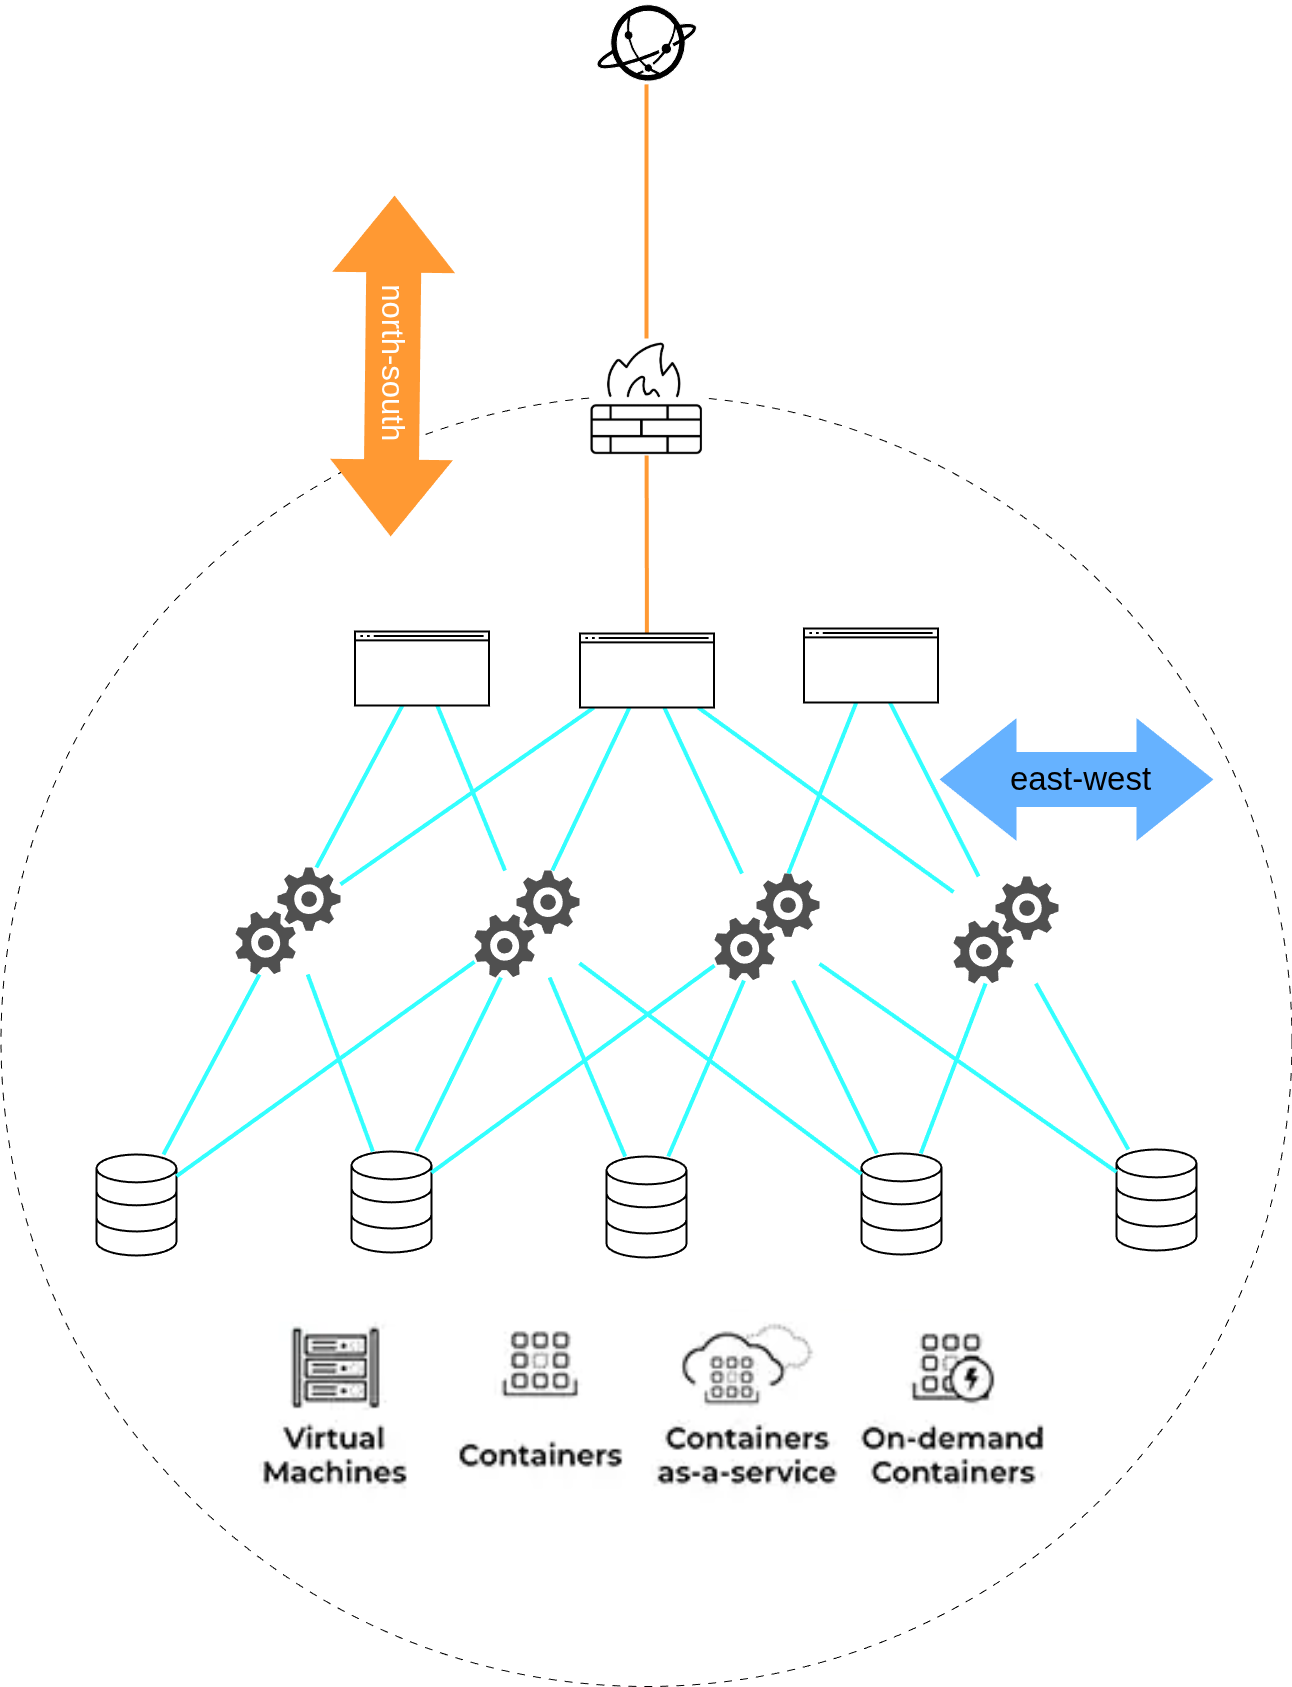
\includegraphics[height=0.8\textheight]{images/nsew.png}
    \caption{Lưu lượng \textit{North-South} (từ Internet vào hệ thống) và \textit{East-West} (giữa các dịch vụ nội bộ)}
    \label{fig:nsew}
\end{figure}

\newpage

\subsection{Các thách thức bảo mật đặc thù của môi trường Kubernetes}

Kubernetes là nền tảng điều phối container tiêu chuẩn, nhưng nó cũng mang lại những thách thức an ninh phức tạp. Môi trường này chứa các thực thể phù du (như \textit{Pod}) có vòng đời rất ngắn, bị xóa sổ và tạo mới liên tục với các địa chỉ IP thay đổi linh hoạt \cite{rice2019kubernetes}. Do đó, việc áp dụng các chính sách bảo mật dựa trên địa chỉ IP tĩnh như mô hình vành đai truyền thống trở nên vô dụng. 

Bên cạnh đó, số lượng danh tính phi con người (\textit{Machine Identities, Workloads, Service Accounts}) giao tiếp với nhau (lưu lượng \textit{East-West}) áp đảo danh tính con người, tạo ra bài toán hóc búa về việc quản lý chuỗi bí mật (\textit{Secret Zero problem}). Nếu không có sự phân đoạn mạng vi mô (\textit{Micro-segmentation}), một container bị chiếm quyền điều khiển có thể trở thành bàn đạp để kẻ tấn công quét mạng và thâm nhập vào các vi dịch vụ trọng yếu khác đang chạy chung trên cùng một cụm.



\subsection{Mục tiêu và phạm vi nghiên cứu}

Nhằm giải quyết những hạn chế của mô hình bảo mật cũ trong kiến trúc phân tán, mục tiêu của nghiên cứu là thiết kế và triển khai \textbf{Kiến trúc Zero Trust (ZTA)} để bảo vệ toàn diện hệ thống Microservices trên môi trường Kubernetes. Phạm vi nghiên cứu tập trung vào:
\begin{itemize}
    \item Áp dụng các công nghệ hiện đại như \textbf{eBPF} (thông qua \textit{Cilium} và \textit{Tetragon} \cite{cilium_docs}) để kiểm soát truy cập tầng mạng và giám sát an ninh tại thời gian thực (\textit{Runtime Security}) mà không làm suy giảm hiệu năng.
    \item Tích hợp \textit{Identity Provider} làm điểm quản trị chính sách xác thực, kết hợp triển khai \textbf{mTLS (Mutual TLS)} nhằm xác thực danh tính hai chiều giữa các dịch vụ.
    \item Xây dựng luồng (pipeline) giám sát và cảnh báo an ninh tập trung (\textit{Observability}) bằng ELK Stack, Prometheus và Grafana.
\end{itemize}

\newpage

\section{Tổng quan về Kiến trúc Zero Trust (ZTA)}

\subsection{Lịch sử hình thành và động lực ra đời}

Khái niệm ``Zero Trust'' (Không tin cậy) lần đầu tiên được định hình bởi nhà phân tích John Kindervag vào năm 2010 khi ông làm việc tại Forrester Research \cite{kindervag2010build}, mặc dù những ý tưởng nền tảng về giải trừ chu vi (\textit{de-perimeterization}) đã được Jericho Forum đề cập từ năm 2004 \cite{jericho2004}. 

Động lực chính dẫn đến sự ra đời của Zero Trust là sự bùng nổ của điện toán đám mây, ứng dụng SaaS và xu hướng làm việc từ xa, khiến ranh giới mạng nội bộ doanh nghiệp không còn tồn tại. Việc phụ thuộc vào ``sự tin cậy ngầm định'' đã tạo điều kiện cho các chiến thuật tấn công dịch chuyển ngang gây ra những vụ rò rỉ dữ liệu thảm khốc. Do đó, Zero Trust ra đời với triết lý cốt lõi: \textit{“Không bao giờ tin cậy, luôn luôn xác minh” (Never trust, always verify)}, yêu cầu mọi kết nối đều phải bị coi là thù địch cho đến khi được xác thực rõ ràng.

% !TEX encoding = UTF-8

\subsection{Các nguyên lý cốt lõi theo NIST SP 800-207}

Viện Tiêu chuẩn và Công nghệ Quốc gia Hoa Kỳ (NIST) đã hệ thống hóa ZTA thông qua ấn phẩm NIST SP 800-207 \cite{rose2020zero} với 7 nguyên lý trọng tâm. Trọng tâm của mô hình này là đặt tài nguyên lên hàng đầu (\textit{Resource-First Security}), cụ thể:

\begin{itemize}
    \item \textbf{Mọi nguồn dữ liệu và dịch vụ điện toán đều là tài nguyên:} \\
    Phạm vi bảo vệ không chỉ dừng lại ở máy chủ vật lý mà bao trùm mọi thiết bị, dịch vụ đám mây (SaaS), vi dịch vụ (Microservices) và hệ thống API. \\
    Ví dụ: Một cổng thông tin nhân sự nội bộ (SaaS) và một API truy vấn cơ sở dữ liệu backend đều được hệ thống ZTA định danh là hai tài nguyên độc lập. Chúng yêu cầu các chính sách kiểm soát quyền truy cập riêng biệt thay vì chỉ được bảo vệ chung bởi một mạng riêng ảo (VPN).

    \item \textbf{Mọi giao tiếp đều phải được bảo mật bất kể vị trí mạng:} \\
    Hệ thống loại bỏ hoàn toàn khái niệm ``vùng tin cậy ẩn'' (\textit{implicit trust zone}). Mọi kết nối nội bộ (trong cùng một trung tâm dữ liệu) hay từ Internet đều phải được mã hóa và xác thực. \\
    Ví dụ: Trong cụm Kubernetes, mặc dù vi dịch vụ \texttt{OrderService} và \texttt{PaymentService} nằm trên cùng một Node nội bộ, lưu lượng giao tiếp giữa chúng vẫn bắt buộc phải được mã hóa và xác thực danh tính hai chiều bằng chứng chỉ số (mTLS) để phòng ngừa bị nghe lén nếu mạng nội bộ bị xâm nhập.

    \item \textbf{Quyền truy cập được cấp trên cơ sở từng phiên làm việc (per-session):} \\
    Tuân thủ nghiêm ngặt nguyên tắc đặc quyền tối thiểu (\textit{Least Privilege}). Sự tin cậy được đánh giá trước khi kết nối và hệ thống chỉ cấp quyền vừa đủ để chủ thể thực hiện một tác vụ cụ thể, sau đó thu hồi ngay. \\
    Ví dụ : Một người dùng được cấp quyền ``Chỉ đọc'' (Read-only) để xem báo cáo tài chính. Nếu người này cố gắng thực hiện lệnh ``Xóa'' (Delete) hoặc chuyển sang xem một tài liệu khác, hệ thống sẽ yêu cầu đánh giá lại quyền hạn cho phiên làm việc mới đó thay vì tiếp tục tin tưởng.

    \item \textbf{Quyền truy cập được xác định bởi chính sách động (dynamic policy):} \\
    Quyết định cấp quyền không dựa trên các quy tắc tĩnh (như dải địa chỉ IP) mà dựa trên việc tổng hợp nhiều tín hiệu ngữ cảnh: danh tính, trạng thái thiết bị, hành vi lịch sử, và vị trí địa lý. \\
    Ví dụ: Một lập trình viên có thể truy cập vào mã nguồn của công ty từ laptop được cấp phát khi đang ngồi tại văn phòng. Tuy nhiên, nếu lập trình viên đó dùng chính tài khoản này nhưng đăng nhập từ mạng Wi-Fi công cộng tại quán cà phê hoặc trên một thiết bị cá nhân không được quản lý, hệ thống động (Policy Engine) sẽ lập tức từ chối truy cập.
    
    \item \textbf{Giám sát và đo lường tính toàn vẹn của mọi tài sản:} \\
    Tổ chức phải liên tục đánh giá trạng thái an ninh của thiết bị. Truy cập sẽ bị từ chối nếu thiết bị có dấu hiệu bị thỏa hiệp hoặc không tuân thủ chính sách bảo mật. \\
    Ví dụ: Hệ thống quản lý thiết bị (MDM) phát hiện laptop của nhân viên chưa cập nhật bản vá lỗ hổng hệ điều hành mới nhất hoặc phần mềm diệt virus đã bị tắt. Ngay lập tức, thiết bị này bị tước quyền truy cập vào các ứng dụng nội bộ cho đến khi hoàn tất việc cập nhật.
    
    \item \textbf{Xác thực và ủy quyền phải linh hoạt và thực thi nghiêm ngặt trước khi truy cập:} \\
    Không chỉ xác thực một lần ở đầu phiên, hệ thống áp dụng xác thực đa yếu tố (MFA) và liên tục tái xác thực (\textit{continuous re-authentication}) trong suốt vòng đời của phiên kết nối. \\
    Ví dụ: Quản trị viên hệ thống đám mây đã đăng nhập thành công vào AWS Console được 2 giờ. Tuy nhiên, khi người này thực hiện một hành động nhạy cảm cao như xóa một \textit{S3 Bucket} chứa dữ liệu người dùng, hệ thống bắt buộc họ phải cắm khóa bảo mật vật lý (YubiKey) hoặc nhập mã sinh trắc học để xác thực lại một lần nữa.

    \item \textbf{Thu thập tối đa thông tin tình báo, nhật ký (Telemetry and Logs):} \\
    Dữ liệu đo từ xa về mạng, thiết bị và hành vi được sử dụng để phân tích, cải thiện tư thế bảo mật và tự động tinh chỉnh chính sách theo thời gian thực. \\
    Ví dụ: Nền tảng phân tích an ninh (SIEM) thu thập nhật ký truy cập và dùng học máy (Machine Learning) để phát hiện một tài khoản nhân sự đột nhiên tải xuống 1.000 hồ sơ ứng viên lúc 2 giờ sáng. Hệ thống tự động kích hoạt kịch bản phản ứng: khóa tạm thời tài khoản và gửi cảnh báo đỏ cho đội ngũ vận hành bảo mật (SOC).
\end{itemize}

\subsection{Năm trụ cột chức năng cốt lõi theo Mô hình CISA ZTMM 2.0}

Để hiện thực hóa 7 nguyên tắc của NIST vào thực tiễn tổ chức, Cơ quan An ninh Mạng và Cơ sở Hạ tầng Hoa Kỳ (CISA) đã phát hành \textit{Mô hình Trưởng thành Zero Trust (ZTMM) phiên bản 2.0} \cite{cisa_ztmm2023}. Mô hình này chia kiến trúc Zero Trust thành 5 trụ cột cấu thành những lĩnh vực bảo vệ thiết yếu, được hỗ trợ bởi 3 năng lực xuyên suốt:

\begin{itemize}
    \item \textbf{Danh tính (Identity):} \\
    Đảm bảo chỉ những người dùng hợp lệ và các thực thể phi nhân sự (máy móc, dịch vụ) mới có quyền truy cập. Yêu cầu thực thi MFA toàn diện và loại bỏ các đặc quyền thường trực (Standing privileges) thông qua cơ chế cấp quyền ``đúng lúc'' (\textit{Just-In-Time - JIT}). \\
    Ví dụ: Thay vì cấp cho quản trị viên cơ sở dữ liệu (DBA) một tài khoản \texttt{root} vĩnh viễn, DBA phải tạo yêu cầu trên hệ thống quản lý danh tính (như HashiCorp Vault). Hệ thống sẽ sinh ra một bộ thông tin đăng nhập tạm thời, chỉ có hiệu lực đúng 60 phút để thực hiện công việc bảo trì, sau đó tự động hủy.
    
    \item \textbf{Thiết bị (Devices):} \\
    Mọi thiết bị (máy chủ, di động, IoT, BYOD) kết nối vào mạng đều phải được kiểm kê và giám sát chặt chẽ về độ tin cậy, trạng thái tuân thủ và mức độ rủi ro theo thời gian thực. \\
    Ví dụ: Triển khai giải pháp EDR (Endpoint Detection and Response) trên mọi máy chủ. Trước khi một máy chủ được phép lấy (pull) mã nguồn từ Gitlab nội bộ, hệ thống phải xác minh qua EDR rằng máy chủ đó không bị nhiễm mã độc.

    \item \textbf{Mạng lưới (Networks):} \\
    Quản lý luồng lưu lượng dựa trên rủi ro thay vì ranh giới vật lý, đồng thời áp dụng rộng rãi các cơ chế phân đoạn mạng vi mô (\textit{Micro-segmentation}) và mã hóa để bảo vệ dữ liệu đang truyền tải. \\
    Ví dụ: Trong môi trường Kubernetes, sử dụng công nghệ eBPF (như \textit{Cilium}) để tạo các quy tắc mạng mức L7: Chỉ cho phép \textit{Frontend Pod} giao tiếp HTTP \texttt{GET} với \textit{Backend Pod} qua cổng \texttt{8080}. Mọi truy cập khác, ví dụ như từ Frontend chọc thẳng vào Database hoặc dùng giao thức khác, đều bị chặn ở mức nhân hệ điều hành (kernel-level).

    \item \textbf{Ứng dụng và Khối lượng công việc (Applications and Workloads):} \\
    Bảo mật lớp phần mềm và môi trường tính toán thông qua kiểm soát truy cập cực kỳ chi tiết (\textit{granular access}) cho cả ứng dụng on-premises và cloud, kết hợp đánh giá cấu hình động. \\
    Ví dụ: Đặt một API Gateway (như \textit{Kong}) ở phía trước các vi dịch vụ. Bất kỳ yêu cầu (request) nào gửi đến API đều phải mang theo một token JWT hợp lệ. API Gateway sẽ giải mã token, kiểm tra chữ ký và đối chiếu quyền (Scope) trước khi định tuyến yêu cầu xuống vi dịch vụ bên dưới.

    \item \textbf{Dữ liệu (Data):} \\
    Đây là mục tiêu bảo vệ tối thượng của ZTA. Dữ liệu phải được phân loại, dán nhãn, mã hóa liên tục (ở cả trạng thái lưu trữ và truyền tải) và tích hợp sâu các công cụ Phòng chống Thất thoát Dữ liệu (DLP) để giám sát trích xuất trái phép. \\
    Ví dụ: Dữ liệu thẻ tín dụng hoặc thông tin cá nhân (PII) của khách hàng trong MySQL được mã hóa minh bạch (TDE). Đồng thời, phần mềm DLP kiểm soát luồng ra internet, chặn đứng ngay lập tức hành vi một nhân viên cố tình đính kèm tệp dữ liệu khách hàng gửi lên Google Drive cá nhân.
\end{itemize}

Ba năng lực xuyên suốt (Cross-cutting capabilities) đóng vai trò kết nối 5 trụ cột trên thành một hệ thống hợp nhất bao gồm: \textbf{Tầm nhìn \& Phân tích (Visibility \& Analytics)}, \textbf{Tự động hóa \& Điều phối (Automation \& Orchestration)}, và \textbf{Quản trị (Governance)}.

\begin{figure}[H]
    \centering
    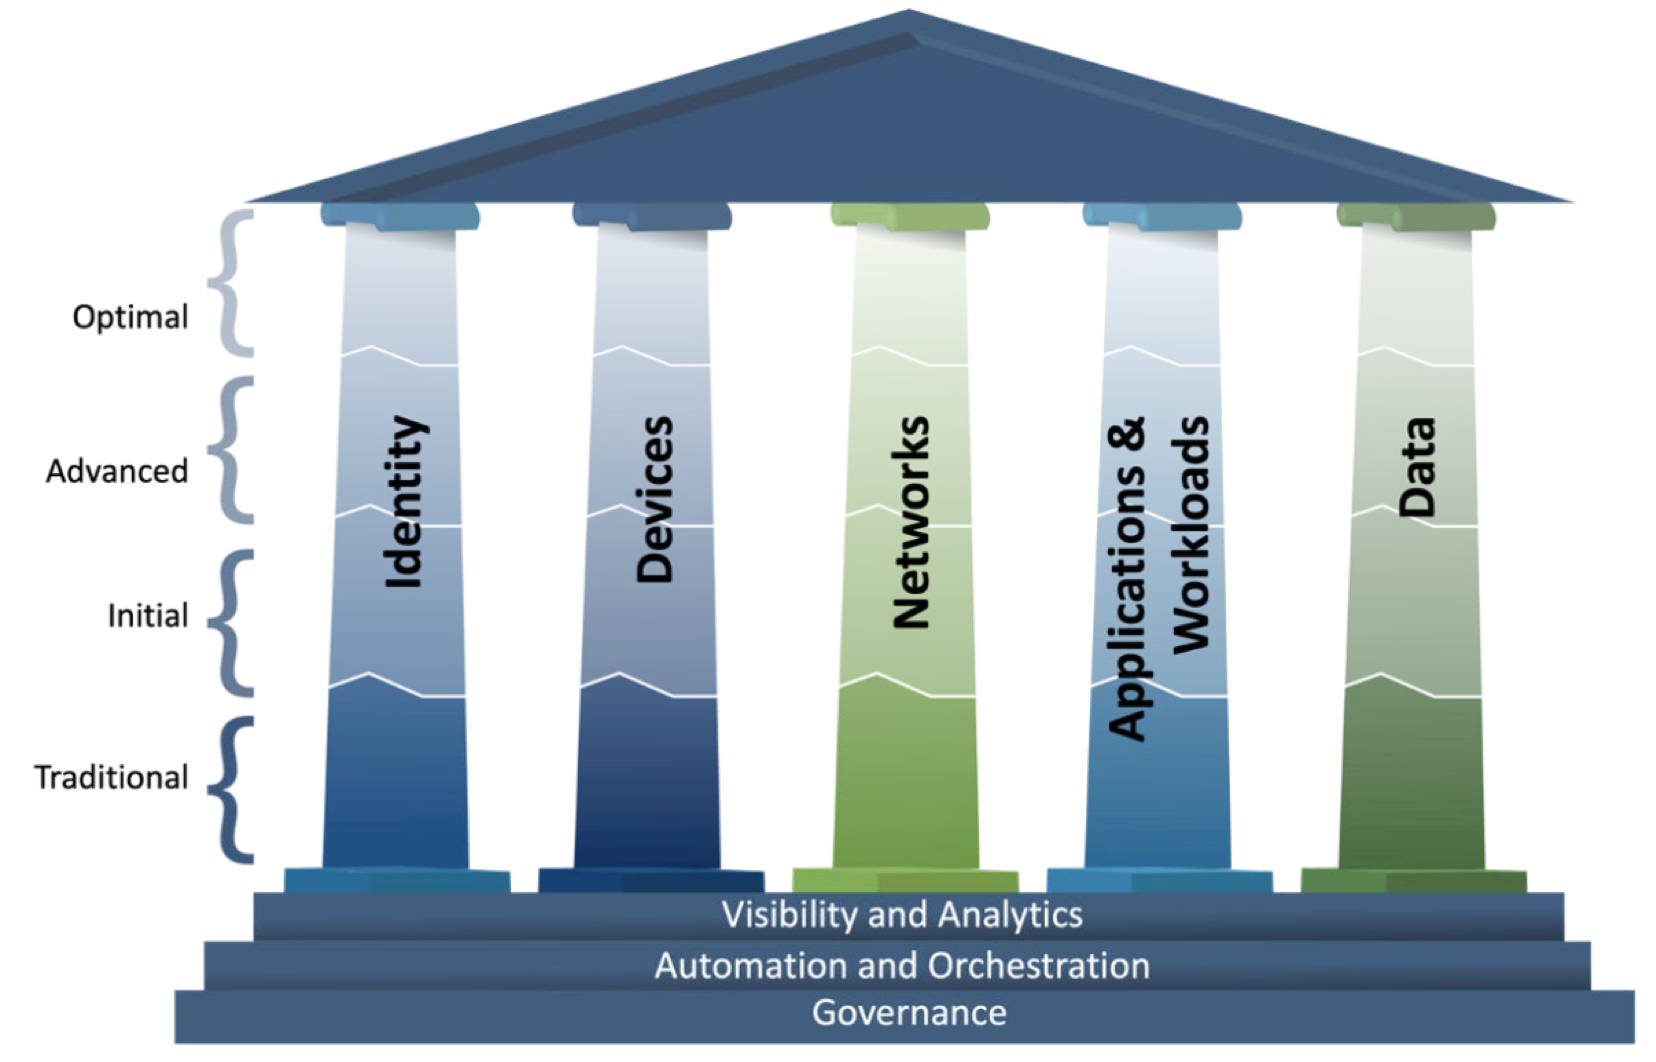
\includegraphics[width=0.9\textwidth]{images/ZTAPillars.png}
    \caption{5 trụ cột của ZTA theo NIST 800 - 207}
    \label{fig:ZTAPillars}
\end{figure}


\subsection{Ba hướng triển khai theo NIST}

Theo tài liệu của NIST \cite[tr. 12--14]{nist800207}, ZTA có thể được triển khai qua ba hướng tiếp cận chính:
\begin{itemize}
    \item \textbf{Enhanced Identity Governance (Quản trị danh tính nâng cao):} Sử dụng danh tính làm thành phần cốt lõi để tạo chính sách. Quyền truy cập vào tài nguyên được cấp dựa trên danh tính và các thuộc tính được gán cho chủ thể đó, trong khi mạng có thể vẫn mở cho mọi kết nối ban đầu.
    \item \textbf{Micro-segmentation (Phân khúc vi mô):} Chống lại kiến trúc mạng ``phẳng'' bằng cách sử dụng tường lửa hoặc cổng thông minh để chia mạng thành các phân đoạn rất nhỏ bao quanh từng tài nguyên hoặc nhóm tài nguyên. Cách này cô lập rủi ro và ngăn chặn triệt để sự di chuyển ngang của kẻ tấn công.
    \item \textbf{Software Defined Perimeter (Chu vi xác định bằng phần mềm - SDP):} Dựa trên cơ sở hạ tầng mạng (thường là mạng lớp 7) để quản lý luồng. Một bộ điều khiển mạng (\textit{Network Controller}) sẽ động thiết lập và cấu hình các đường truyền an toàn giữa máy khách và tài nguyên dựa trên quyết định từ Động cơ chính sách.
\end{itemize}

\subsection{So sánh ZTA với mô hình Perimeter-based Security}

Sự khác biệt giữa Kiến trúc Zero Trust và Mô hình bảo mật vành đai truyền thống được thể hiện rõ rệt qua cách tiếp cận với sự tin cậy và quyền truy cập (Bảng \ref{tab:zta_vs_perimeter}). Mô hình ZTA khắc phục triệt để các lỗ hổng của kiến trúc cũ, đặc biệt trong việc ngăn ngừa tấn công dịch chuyển ngang.

\begin{table}[htbp]
\centering
\caption{So sánh Mô hình bảo mật vành đai và Kiến trúc Zero Trust}
\label{tab:zta_vs_perimeter}
\begin{tabularx}{\textwidth}{|l|X|X|}
\hline
\rowcolor[HTML]{EFEFEF}
\textbf{Tiêu chí} & \textbf{Mô hình vành đai (Perimeter-based)} & \textbf{Kiến trúc Zero Trust (ZTA)} \\ \hline
\textbf{Giả định tin cậy} & Tin tưởng mặc định mọi thực thể bên trong mạng nội bộ. & Không tin tưởng bất kỳ thực thể nào, bất kể vị trí vật lý hay vị trí mạng. \\ \hline
\textbf{Cơ chế xác thực} & Xác thực tĩnh một lần tại thời điểm đăng nhập (tại cổng vào). & Đánh giá rủi ro động, xác thực liên tục và cấp quyền theo từng phiên giao dịch. \\ \hline
\textbf{Quyết định truy cập} & Dựa vào các thông tin tĩnh (ví dụ: địa chỉ IP, dải mạng). & Dựa trên danh tính xác thực mạnh, bối cảnh môi trường và mức độ rủi ro của thiết bị. \\ \hline
\textbf{Chống dịch chuyển ngang} & Vô cùng yếu kém. Tin tặc dễ dàng di chuyển khi đã thâm nhập thành công. & Vô hiệu hóa thành công nhờ xác thực độc lập từng tài nguyên và phân đoạn mạng vi mô. \\ \hline
\end{tabularx}
\end{table}
% !TEX encoding = UTF-8

\chapter{Cơ sở lý thuyết}

\section{Khái niệm 1}
Trình bày các định nghĩa, lý thuyết, công nghệ nền tảng.
Ví dụ: Tham khảo từ \parencite{example_article_2023}.

\section{Công nghệ và Công cụ}
Giới thiệu các ngôn ngữ lập trình, framework, hệ quản trị cơ sở dữ liệu sẽ dùng.

\section{Các nghiên cứu liên quan}
Đánh giá ưu nhược điểm của các giải pháp, nghiên cứu trước đây.

% !TEX encoding = UTF-8
\chapter{Xây dựng hệ thống Tuyển dụng trực tuyến}

\section{Phân tích yêu cầu nghiệp vụ}

\subsection{Khảo sát và thu thập yêu cầu nghiệp vụ}
Để xây dựng một quy trình nghiệp vụ chuẩn hóa và phù hợp với thực tiễn, đồ án đã tiến hành tham khảo mô hình hoạt động của các nền tảng tuyển dụng uy tín.
Đối với phân hệ quản lý tin đăng và tìm kiếm việc làm (Job Portal), đồ án tham khảo quy trình tiếp cận ứng viên của các mạng lưới phổ biến như LinkedIn \cite{linkedin_recruiter} và Indeed \cite{indeed_hiring}. Tại thị trường Việt Nam, các quy trình về đăng tuyển và quản lý hồ sơ ứng viên được tham chiếu theo mô hình của TopCV \cite{topcv_vn} và VietnamWorks \cite{vietnamworks} để đảm bảo tính phù hợp với người dùng trong nước.
Đặc biệt, đối với phân hệ quản trị tuyển dụng (Hiring Service/ATS), chức năng quản lý ứng viên theo quy trình (Pipeline) và bảng điều khiển (Kanban Board) được thiết kế dựa trên nguyên lý của các hệ thống ATS chuyên nghiệp như Greenhouse \cite{greenhouse_ats} và SmartRecruiters \cite{smartrecruiters}. Việc tham khảo này giúp hệ thống Job7189 không chỉ dừng lại ở việc đăng tin mà còn hỗ trợ doanh nghiệp quản lý trọn vẹn vòng đời tuyển dụng.

Việc khảo sát tập trung vào các nội dung chính:
\begin{itemize}
    \item Luồng đăng tuyển và quản lý tin tuyển dụng.
    \item Luồng ứng tuyển và xử lý hồ sơ ứng viên.
    \item Cách các hệ thống hiện tại quản lý trạng thái tin tuyển dụng và hồ sơ.
    \item Quy trình phối hợp giữa các vai trò: Recruiter, Hiring Manager, HR, Admin và Ứng viên.
\end{itemize}

Kết quả khảo sát cho thấy, mặc dù mỗi nền tảng có cách triển khai riêng, nhưng đa số các hệ thống đều tuân theo các luồng nghiệp vụ chung:
\begin{itemize}
    \item Tin tuyển dụng được khởi tạo, chỉnh sửa, gửi duyệt, công bố và kết thúc theo vòng đời trạng thái;
    \item Hồ sơ ứng viên được tiếp nhận, sàng lọc, phỏng vấn, đánh giá và cập nhật kết quả theo quy trình nhiều bước;
    \item Mọi thay đổi quan trọng đều được ghi nhận lịch sử để phục vụ theo dõi, báo cáo và đối soát dữ liệu;
    \item Các vai trò tham gia được phân quyền rõ ràng trong từng giai đoạn của quy trình.
\end{itemize}

Trên cơ sở các luồng và quy trình nghiệp vụ thu được từ khảo sát, đồ án tiến hành xây dựng hệ thống tuyển dụng với mục tiêu chuẩn hóa quy trình, kiểm soát chặt chẽ vòng đời dữ liệu và đảm bảo tính nhất quán trong toàn bộ hoạt động tuyển dụng. Dựa trên các nghiên cứu về quy trình tuyển dụng hiệu quả \cite{smart2008} và khảo sát các nền tảng thực tế.

\subsection{Mô hình hóa quy trình nghiệp vụ (BPMN)}
Dựa trên quá trình khảo sát các hệ thống thực tế, đồ án mô hình hóa các quy trình nghiệp vụ cốt lõi của hệ thống tuyển dụng. Mục tiêu là làm rõ cách thức vận hành thực tế, các vai trò tham gia, cũng như các quy tắc nghiệp vụ chi phối vòng đời của dữ liệu trong hệ thống. Trong đó, Quy trình Đăng tuyển (Job Posting Lifecycle) được xác định là quy trình trung tâm, ảnh hưởng trực tiếp đến toàn bộ hoạt động của nền tảng tuyển dụng.

\subsubsection{Quy trình Đăng tuyển}
\begin{figure}[htbp]
    \centering
    \includegraphics[width=1\textwidth]{images/dangtuyen.png}
    \caption{Sơ đồ Quy trình Đăng tuyển}
    \label{fig:bpmn_dang_tuyen}
\end{figure}

\textbf{1. Giai đoạn soạn thảo} \\
Mô tả nghiệp vụ: Người phụ trách việc đăng bài khởi tạo một tin tuyển dụng mới và nhập các thông tin mô tả công việc (Job Description): tiêu đề công việc, mô tả nhiệm vụ, yêu cầu ứng viên, mức lương, địa điểm làm việc, hình thức làm việc, thời hạn ứng tuyển và các thông tin liên quan khác. Sau khi được tạo, tin tuyển dụng được lưu ở trạng thái DRAFT và chỉ hiển thị với những người có quyền truy cập. 

Tại giai đoạn này, hệ thống không cho phép xóa tin tuyển dụng trong bất kỳ trường hợp nào, kể cả khi tin mới được tạo và chưa gửi duyệt. Thay vì cơ chế xóa, hệ thống áp dụng mô hình quản lý vòng đời bằng chuyển trạng thái và lưu trữ (Archive) nhằm:
\begin{itemize}
    \item Bảo toàn dữ liệu nghiệp vụ.
    \item Đảm bảo khả năng truy vết lịch sử xử lý tin.
    \item Duy trì sự liên kết giữa tin tuyển dụng và các dữ liệu phát sinh như hồ sơ ứng viên, báo cáo và thống kê.
\end{itemize}
Trong giai đoạn soạn thảo, người phụ trách tuyển dụng được phép: Chỉnh sửa nội dung tin, Lưu trữ tạm thời tin nếu chưa tiếp tục xử lý, Gửi tin để chuyển sang giai đoạn kiểm duyệt.

\textbf{2. Giai đoạn gửi duyệt} \\
Mô tả nghiệp vụ: Khi nội dung tin đã được hoàn thiện, người phụ trách tuyển dụng thực hiện thao tác Submit. Hệ thống tiếp nhận yêu cầu và chuyển tin sang trạng thái PENDING. Tại thời điểm này, nội dung tin không được phép chỉnh sửa nhằm đảm bảo tính nhất quán trong suốt quá trình kiểm tra. Trong trường hợp phát hiện sai sót, người phụ trách tuyển dụng có thể hủy gửi duyệt để đưa tin quay lại giai đoạn soạn thảo và tiếp tục chỉnh sửa.

\textbf{3. Giai đoạn kiểm duyệt} \\
Mô tả nghiệp vụ: Bộ phận quản trị nền tảng tiến hành rà soát các tin đang chờ duyệt từ các đơn vị khác nhau theo các quy chuẩn đã được thiết lập trước. Sau khi đánh giá, nội dung tin sẽ được xử lý theo một trong hai hướng:
\begin{itemize}
    \item Chấp thuận: Tin được cho phép công bố trên hệ thống.
    \item Từ chối: Tin bị yêu cầu chỉnh sửa lại nội dung và gửi duyệt lại.
\end{itemize}

\textbf{4. Giai đoạn vận hành và kết thúc} \\
Mô tả nghiệp vụ: Các tin đã được chấp thuận sẽ được hiển thị công khai cho ứng viên trong thời gian hiệu lực. Tin tuyển dụng kết thúc khi: Hết thời hạn đăng tuyển; Doanh nghiệp chủ động ngừng hiển thị tin; Admin của hệ thống gỡ tin. Các tin kết thúc được lưu trữ để phục vụ công tác báo cáo, thống kê và đối soát dữ liệu trong tương lai.

\subsubsection{Quy trình Ứng tuyển}
Quy trình Ứng tuyển mô tả toàn bộ hành trình của một ứng viên kể từ khi tiếp cận tin tuyển dụng cho đến khi nhận được kết quả cuối cùng từ phía doanh nghiệp. Quy trình này kết nối trực tiếp giữa người tìm việc và tổ chức tuyển dụng, đồng thời tạo ra chuỗi dữ liệu đầu vào quan trọng cho các hoạt động sàng lọc, phỏng vấn và ra quyết định tuyển dụng.

\begin{figure}[htbp]
    \centering
        \includegraphics[width=1\textwidth]{images/ungtuyen.png}
    \caption{Sơ đồ Quy trình Ứng tuyển}
    \label{fig:bpmn_ung_tuyen}
\end{figure}

\textbf{1. Giai đoạn Tìm kiếm \& Tiếp cận việc làm} \\
Mô tả nghiệp vụ: Người tìm việc truy cập cổng thông tin tuyển dụng (Job Portal) và sử dụng các chức năng tìm kiếm, lọc, sắp xếp để tra cứu các vị trí tuyển dụng phù hợp theo nhiều tiêu chí như: ngành nghề, địa điểm, mức lương, hình thức làm việc và kinh nghiệm yêu cầu. Tại giai đoạn này, người dùng có thể xem chi tiết nội dung tin tuyển dụng, thông tin doanh nghiệp và các yêu cầu liên quan trước khi quyết định ứng tuyển.

\textbf{2. Giai đoạn Ứng tuyển} \\
Mô tả nghiệp vụ: Khi quyết định ứng tuyển, ứng viên thực hiện thao tác nộp hồ sơ. Hệ thống cho phép ứng viên: Tải lên CV từ thiết bị cá nhân hoặc chọn từ hồ sơ đã lưu trước đó, bổ sung các thông tin cần thiết theo mẫu ứng tuyển. Hồ sơ của ứng viên được lưu trữ trên hệ thống lưu trữ tập trung (Storage Service) và hệ thống đồng thời tạo một bản ghi Application gắn với tin tuyển dụng tương ứng, chính thức ghi nhận việc ứng tuyển của ứng viên.

\textbf{3. Giai đoạn Sàng lọc \& Phỏng vấn} \\
Mô tả nghiệp vụ: Sau khi tiếp nhận hồ sơ, đội ngũ tuyển dụng tiến hành xem xét danh sách ứng viên cho từng vị trí. Recruiter và Hiring Manager đánh giá hồ sơ dựa trên các tiêu chí chuyên môn và yêu cầu công việc. Đối với các hồ sơ phù hợp, bộ phận điều phối tuyển dụng (Coordinator) thực hiện liên hệ và lên lịch phỏng vấn. Quá trình phỏng vấn được thực hiện bởi các Interviewer, trong đó kết quả đánh giá và nhận xét được ghi nhận trực tiếp vào hệ thống. Quy trình này có thể bao gồm nhiều vòng phỏng vấn và các hoạt động đánh giá bổ sung tùy theo chính sách tuyển dụng của từng tổ chức.

\textbf{4. Giai đoạn Kết quả \& Thông báo} \\
Mô tả nghiệp vụ: Sau khi hoàn tất các vòng đánh giá, hệ thống cập nhật trạng thái cuối cùng của hồ sơ ứng viên: Offer đối với ứng viên đạt yêu cầu, Reject đối với các hồ sơ không phù hợp. Kết quả này được thông báo đến ứng viên thông qua các kênh liên lạc của hệ thống như email hoặc thông báo trên nền tảng, đồng thời được lưu trữ để phục vụ mục đích báo cáo và thống kê trong tương lai.

\subsection{Biểu đồ Use Case và Đặc tả chức năng}

Biểu đồ Use Case tổng quát của hệ thống Job7189 được thiết kế dựa trên các ký pháp tiêu chuẩn của Ngôn ngữ Mô hình hóa Thống nhất (UML) theo hướng dẫn của Fowler \cite{fowler2003}. Quá trình xác định các tác nhân (Actors) và ca sử dụng (Use Cases) tuân thủ phương pháp phân tích thiết kế hướng đối tượng được đề xuất bởi Larman \cite{larman2004}, nhằm đảm bảo bao quát đầy đủ các tương tác giữa người dùng và hệ thống.

\begin{figure}[H]
    \centering

    \begin{subfigure}{0.48\textwidth}
        \centering
        \includegraphics[width=\linewidth]{images/uc1}
        \caption{Phần 1}
    \end{subfigure}
    \hfill
    \begin{subfigure}{0.48\textwidth}
        \centering
        \includegraphics[width=\linewidth]{images/uc2}
        \caption{Phần 2}
    \end{subfigure}

    \caption{Biểu đồ Use Case hệ thống tuyển dụng}
    \label{fig:usecase_join}
\end{figure}

\subsubsection{Danh sách tác nhân hệ thống (Actors)}

Hệ thống phân định rõ ràng trách nhiệm của từng vai trò tham gia vào quy trình tuyển dụng. Việc phân chia chi tiết giữa các vai trò như \textit{Recruiter}, \textit{Hiring Manager} và \textit{Interviewer} được thiết kế dựa trên nguyên lý tuyển dụng "Who: The A Method" \cite{smart2008} nhằm đảm bảo tính khách quan và hiệu quả.

Dưới đây là danh sách chi tiết các tác nhân trong hệ thống:

\begin{table}[H]
    \centering
    \renewcommand{\arraystretch}{1.3} % Tăng khoảng cách dòng cho dễ đọc
    \caption{Đặc tả các tác nhân và quyền hạn trong hệ thống}
    \label{tab:actors_list}
    \small % Dùng font nhỏ hơn một chút để bảng gọn gàng
    \begin{tabular}{|c|p{3.5cm}|p{9.5cm}|}
        \hline
        \textbf{STT} & \textbf{Tác nhân (Actor)} & \textbf{Mô tả chi tiết} \\
        \hline
        1 & \textbf{System Admin} & Quản trị viên cấp cao nhất. Quản lý toàn bộ nền tảng (multi-tenancy), bao gồm quản lý các workspace, kiểm duyệt tin đăng công khai và cấu hình tham số toàn cục. \\
        \hline
        2 & \textbf{Workspace Admin} & Quản trị viên của một công ty (tenant). Chịu trách nhiệm cấu hình workspace, mời thành viên, phân quyền và giám sát hoạt động tuyển dụng của công ty. \\
        \hline
        3 & \textbf{RecOps} & Chuyên viên vận hành tuyển dụng. Người thiết kế luồng quy trình (Pipeline), tạo mẫu đánh giá (Scorecard), cấu hình automation và email template. \\
        \hline
        4 & \textbf{Recruiter} & Chuyên viên tuyển dụng toàn trình. Người "sở hữu" ứng viên, chịu trách nhiệm đăng tin, sàng lọc (sourcing), quản lý ứng viên qua các vòng và gửi Offer. \\
        \hline
        5 & \textbf{Coordinator} & Điều phối viên. Chịu trách nhiệm về logistics: lên lịch phỏng vấn, đặt phòng họp và gửi thư mời. Không tham gia vào quyết định tuyển dụng. \\
        \hline
        6 & \textbf{Hiring Manager} & Trưởng bộ phận cần tuyển (người ra quyết định). Tạo yêu cầu tuyển dụng (Requisition), tham gia phỏng vấn và phê duyệt Offer cuối cùng. \\
        \hline
        7 & \textbf{Interviewer} & Người phỏng vấn. Bất kỳ nhân viên nào được mời tham gia đánh giá ứng viên. Hệ thống áp dụng cơ chế "Independent Feedback" (không được xem đánh giá của người khác trước khi nộp đánh giá của mình). \\
        \hline
        8 & \textbf{Member} & Nhân viên thông thường. Có thể xem tin tuyển dụng nội bộ, giới thiệu ứng viên (Referral) và quản lý hồ sơ cá nhân. \\
        \hline
        9 & \textbf{Guest} & Khách vãng lai chưa đăng nhập. Chỉ có quyền xem danh sách việc làm công khai (Job Board) và tìm kiếm thông tin. \\
        \hline
        10 & \textbf{Candidate} & Ứng viên đã đăng ký tài khoản. Có quyền quản lý hồ sơ (CV), ứng tuyển (Apply), theo dõi trạng thái đơn và thực hiện các quyền riêng tư dữ liệu. \\
        \hline
        11 & \textbf{User} & Thực thể cơ sở (Base User) trong hệ thống định danh. Mọi tác nhân (trừ Guest) đều kế thừa từ User để thực hiện các chức năng đăng nhập, đăng xuất và bảo mật tài khoản. \\
        \hline
    \end{tabular}
\end{table}

% !TEX encoding = UTF-8

\subsection{Đặc tả chi tiết các Use Case cốt lõi}
Dưới đây là đặc tả chi tiết cho 03 hành động quan trọng nhất, thể hiện tính phối hợp giữa các dịch vụ và các kịch bản xử lý ngoại lệ trong kiến trúc Microservices của hệ thống \textbf{job7189}.

% --- USE CASE 1 ---
\subsubsection*{Use Case 1: Ứng tuyển việc làm (Job Application)}
\textit{Mô tả kịch bản ứng viên nộp hồ sơ vào một vị trí công việc đang mở.}

\begin{center}
\renewcommand{\arraystretch}{1.4} % Giãn dòng trong bảng cho dễ đọc
\small
\begin{tabular}{|p{3.5cm}|p{12cm}|}
\hline
\rowcolor[HTML]{EFEFEF} 
\textbf{Thành phần} & \textbf{Mô tả chi tiết} \\ \hline
\textbf{Tác nhân} & Ứng viên (Candidate). \\ \hline
\textbf{Mục tiêu} & Gửi hồ sơ CV và khởi tạo đơn ứng tuyển tại Hiring Service. \\ \hline
\textbf{Tiền điều kiện} & Ứng viên đã đăng nhập; Tin tuyển dụng đang ở trạng thái \texttt{PUBLISHED}. \\ \hline
\textbf{Luồng chính} & 
1. Ứng viên chọn tệp CV và nhấn nút "Ứng tuyển". \newline
2. Hệ thống lấy \textit{Presigned URL} từ \textit{Storage Service} và tải file lên \textit{MinIO}. \newline
3. \textit{Candidate Service} lưu đường dẫn tệp (\textit{FilePath}) và tạo \textit{ResumeID}. \newline
4. \textit{Hiring Service} gọi sang \textit{Job Service} để kiểm tra trạng thái tin đăng. \newline
5. Hệ thống tạo bản ghi \textit{JobApplication} và phát sự kiện tạo đơn vào Kafka. \\ \hline
\textbf{Luồng thay thế} & 
4a. Nếu \textit{Job Service} phản hồi tin đăng đã đóng (\texttt{CLOSED}) hoặc hết hạn: Hệ thống thông báo lỗi và hủy quy trình ứng tuyển. \newline
2a. Nếu việc tải tệp lên \textit{MinIO} thất bại: Thông báo lỗi kết nối và yêu cầu thử lại. \\ \hline
\textbf{Hậu điều kiện} & Đơn ứng tuyển hiển thị trong danh sách của nhà tuyển dụng; Ứng viên nhận email xác nhận. \\ \hline
\end{tabular}
\end{center}

\vspace{0.8cm} % Tạo khoảng cách hợp lý giữa 2 Use Case

\newpage
% --- USE CASE 2 ---
\subsubsection*{Use Case 2: Quản lý Tin tuyển dụng (Job Posting Lifecycle)}
\textit{Mô tả quy trình soạn thảo và gửi duyệt nội dung tin đăng của nhà tuyển dụng.}

\begin{center}
\renewcommand{\arraystretch}{1.4}
\small
\begin{tabular}{|p{3.5cm}|p{12cm}|}
\hline
\rowcolor[HTML]{EFEFEF} 
\textbf{Thành phần} & \textbf{Mô tả chi tiết} \\ \hline
\textbf{Tác nhân} & Nhà tuyển dụng (Recruiter). \\ \hline
\textbf{Mục tiêu} & Hoàn thiện nội dung JD và chuyển trạng thái sang chờ phê duyệt. \\ \hline
\textbf{Tiền điều kiện} & Nhà tuyển dụng có quyền \texttt{CREATE\_JOB} trong Workspace hiện tại. \\ \hline
\textbf{Luồng chính} & 
1. Nhà tuyển dụng nhập thông tin JD (Tiêu đề, lương, yêu cầu...). \newline
2. Hệ thống lưu bản ghi vào bảng \texttt{job\_jds} với trạng thái \texttt{DRAFT}. \newline
3. Nhà tuyển dụng nhấn nút "Gửi duyệt" (Submit). \newline
4. \textit{Job Service} chuyển trạng thái thành \texttt{PENDING} và khóa quyền chỉnh sửa nội dung. \newline
5. Hệ thống ghi nhận lịch sử phiên bản vào bảng \texttt{job\_histories}. \\ \hline
\textbf{Luồng thay thế} & 
3a. Nhà tuyển dụng chọn "Lưu tạm": Hệ thống giữ tin ở trạng thái \texttt{DRAFT} để có thể chỉnh sửa sau. \newline
4a. Nếu các thông tin bắt buộc bị thiếu: Hệ thống báo lỗi và yêu cầu bổ sung trước khi Submit. \\ \hline
\textbf{Hậu điều kiện} & Tin tuyển dụng xuất hiện trong danh sách chờ duyệt của Quản trị viên (Admin). \\ \hline
\end{tabular}
\end{center}

\vspace{0.8cm}

\newpage
% --- USE CASE 3 ---
\subsubsection*{Use Case 3: Di chuyển trạng thái ứng viên (Move Candidate Stage)}
\textit{Mô tả kịch bản nhà tuyển dụng điều phối ứng viên qua các vòng tuyển dụng trên Kanban.}

\begin{center}
\renewcommand{\arraystretch}{1.4}
\small
\begin{tabular}{|p{3.5cm}|p{12cm}|}
\hline
\rowcolor[HTML]{EFEFEF} 
\textbf{Thành phần} & \textbf{Mô tả chi tiết} \\ \hline
\textbf{Tác nhân} & Nhà tuyển dụng (Recruiter). \\ \hline
\textbf{Mục tiêu} & Cập nhật vòng tuyển dụng cho ứng viên và kích hoạt thông báo tự động. \\ \hline
\textbf{Tiền điều kiện} & Nhà tuyển dụng đang xem bảng Kanban của một tin tuyển dụng cụ thể. \\ \hline
\textbf{Luồng chính} & 
1. Nhà tuyển dụng kéo thẻ ứng viên từ cột hiện tại sang cột trạng thái mới. \newline
2. \textit{Hiring Service} gọi sang \textit{Identity Service} kiểm tra quyền hạn của người dùng. \newline
3. Hệ thống cập nhật \texttt{StageID} mới vào cơ sở dữ liệu. \newline
4. \textit{Hiring Service} phát sự kiện \texttt{app.moved} vào Message Broker. \newline
5. \textit{Communication Service} tiêu thụ sự kiện và tự động gửi email cho ứng viên. \\ \hline
\textbf{Luồng thay thế} & 
2a. Nếu \textit{Identity Service} phản hồi người dùng không có quyền (\texttt{403 Forbidden}): Hệ thống trả thẻ ứng viên về vị trí cũ và thông báo từ chối truy cập. \newline
5a. Nếu dịch vụ Email bị lỗi: Sự kiện vẫn được lưu tại Kafka để xử lý lại (Retry) sau khi dịch vụ phục hồi. \\ \hline
\textbf{Hậu điều kiện} & Trạng thái mới của ứng viên được đồng bộ hóa trên giao diện tất cả người dùng liên quan. \\ \hline
\end{tabular}
\end{center}





\subsubsection*{Danh sách vai trò và chức năng trong hệ thống}
\label{tab:roles_permissions}
\begin{tabularx}{\textwidth}{|l|l|X|X|}
\hline
\rowcolor[HTML]{EFEFEF} 
\textbf{Nhóm} & \textbf{Vai trò} & \textbf{Mô tả vai trò} & \textbf{Chức năng chính} \\ \hline
Platform & System Admin & Quản trị toàn bộ nền tảng, kiểm soát nội dung và tenant & Duyệt tin (Approve/Reject), quản lý danh mục, quản lý Workspace \\ \hline
Workspace & Workspace Admin & Quản trị doanh nghiệp & Cấu hình công ty, mua gói dịch vụ, phân quyền \\ \cline{2-4} 
 & RecOps & Thiết kế và tối ưu quy trình & Cấu hình pipeline, email template, scorecard \\ \cline{2-4} 
 & Hiring Manager & Chủ sở hữu nhu cầu tuyển dụng & Tạo Requisition, phê duyệt kế hoạch, quyết định Offer \\ \cline{2-4} 
 & Recruiter & Vận hành quy trình tuyển dụng & Sourcing, đăng tin, sàng lọc hồ sơ \\ \cline{2-4} 
 & Coordinator & Điều phối phỏng vấn & Lên lịch phỏng vấn, sắp xếp phòng \\ \cline{2-4} 
 & Interviewer & Đánh giá ứng viên & Tham gia phỏng vấn, chấm điểm bằng Scorecard \\ \cline{2-4} 
 & Member & Thành viên workspace & Xem thông tin nội bộ, giới thiệu ứng viên (Referral) \\ \hline
Public & Guest & Người dùng chưa đăng nhập & Xem tin tuyển dụng, tìm kiếm việc làm \\ \cline{2-4} 
 & Candidate & Người tìm việc đã đăng ký & Ứng tuyển, quản lý CV, theo dõi đơn \\ \cline{2-4} 
 & User & Tài khoản hệ thống cơ bản & Quản lý tài khoản, đăng nhập SSO \\ \hline
\end{tabularx}
\end{table}

\subsection{Yêu cầu phi chức năng}
Bên cạnh các yêu cầu nghiệp vụ, hệ thống còn phải đáp ứng các yêu cầu phi chức năng nhằm đảm bảo khả năng vận hành ổn định, an toàn, mở rộng và hiệu quả trong môi trường thực tế. Các yêu cầu này đóng vai trò nền tảng cho việc lựa chọn kiến trúc và công nghệ triển khai hệ thống.

\textbf{1. Kiến trúc hệ thống} \\
Hệ thống được thiết kế theo mô hình Microservices kết hợp Event-Driven Architecture nhằm:
\begin{itemize}
    \item Tách biệt các chức năng nghiệp vụ thành các dịch vụ độc lập.
    \item Giảm sự phụ thuộc chặt chẽ giữa các thành phần.
    \item Tăng khả năng mở rộng và khả năng bảo trì.
    \item Cho phép hệ thống phản ứng linh hoạt với các sự kiện nghiệp vụ phát sinh trong quá trình vận hành.
\end{itemize}
Mô hình Event-Driven giúp các dịch vụ giao tiếp bất đồng bộ thông qua các sự kiện, từ đó giảm coupling và tăng khả năng chịu tải của toàn hệ thống.

\textbf{2. Bảo mật và phân quyền} \\
\textit{Authentication – Xác thực:} Hệ thống sử dụng Keycloak như một Identity Provider (IdP) trung tâm để quản lý danh tính người dùng. Keycloak chịu trách nhiệm: Xác thực người dùng thông qua cơ chế Single Sign-On (SSO); Cấp phát các Token xác thực (Access Token, Refresh Token, ID Token); Quản lý vòng đời phiên đăng nhập và chính sách bảo mật. \\
\textit{Authorization – Phân quyền:} Hệ thống áp dụng mô hình Token Exchange / JWT Enrichment nhằm tối ưu hóa hiệu năng và tăng tính độc lập của các Microservice. Quy trình phân quyền được tổ chức như sau: Identity Service chịu trách nhiệm tổng hợp và đóng gói toàn bộ thông tin Role và Permission của người dùng vào Access Token. Các Microservice nghiệp vụ khi nhận request chỉ cần giải mã và kiểm tra Token để thực hiện Authorization Enforcement. Việc kiểm tra quyền được thực hiện hoàn toàn Stateless, không yêu cầu truy vấn Database hay gọi ngược về Identity Service.

\textbf{3. Bảo mật dữ liệu} \\
Đối với dữ liệu tập tin (CV, tài liệu ứng tuyển…), hệ thống áp dụng cơ chế Presigned URL khi tải lên hoặc tải xuống file. Theo đó: Client chỉ được cấp quyền truy cập file trong thời gian giới hạn; Không cho phép truy cập trực tiếp vào hệ thống lưu trữ; Giảm thiểu nguy cơ rò rỉ dữ liệu và tấn công trái phép.

\textbf{4. Hiệu năng} \\
Hệ thống được tối ưu hóa về độ trễ và khả năng xử lý tải lớn thông qua: Cơ chế Stateless Authorization giúp kiểm tra quyền với độ trễ gần như bằng không; Giao tiếp bất đồng bộ trong kiến trúc Event-Driven; Khả năng mở rộng linh hoạt của các Microservice.

\textbf{5. Tính sẵn sàng và độ tin cậy} \\
Hệ thống được triển khai trên nền tảng Kubernetes, cho phép: Tự động phát hiện lỗi và khởi động lại dịch vụ gặp sự cố; Cân bằng tải giữa các instance; Mở rộng hoặc thu hẹp tài nguyên theo nhu cầu sử dụng.

\section{Thiết kế kiến trúc hệ thống}
Để trực quan hóa kiến trúc hệ thống từ mức tổng quan đến chi tiết, đồ án áp dụng mô hình C4 (Context, Containers, Components, Code).

\subsection{Level 1: Sơ đồ ngữ cảnh hệ thống}
Sơ đồ ngữ cảnh cung cấp cái nhìn tổng quan nhất về hệ thống Job7189, đặt nó vào trong môi trường hoạt động thực tế và xác định các mối tương tác với người dùng và các hệ thống bên ngoài.

\begin{figure}[H]
    \centering
    \includegraphics[width=0.5\textwidth]{images/structurizr-1-1_SystemContext-key.png}
    \caption{Quy ước ký hiệu sử dụng trong các sơ đồ của hệ thống}
    \label{fig:c4-notation}
\end{figure}

\begin{figure}[H]
    \centering
    \includegraphics[width=0.8\textwidth]{images/structurizr-1-1_SystemContext.png}
    \caption{Sơ đồ ngữ cảnh hệ thống của hệ thống Job7189}
    \label{fig:system-context}
\end{figure}


\textbf{1. Trung tâm hệ thống: Job7189 System} \\
Job7189 là hệ thống phần mềm lõi được xây dựng nhằm hỗ trợ và tự động hóa toàn bộ quy trình tuyển dụng cho doanh nghiệp. Trách nhiệm chính của Job7189 bao gồm: Quản lý tin tuyển dụng; Tiếp nhận và xử lý hồ sơ ứng viên; Hỗ trợ sàng lọc, phỏng vấn, đánh giá; Quản lý quy trình theo pipeline; Cung cấp báo cáo thống kê.

\textbf{2. Người dùng (Users):}
\begin{itemize}
    \item \textbf{Internal Users:} Bao gồm các vai trò như Workspace Admin, Recruiter, Hiring Manager, Interviewer. Họ tương tác với hệ thống để thực hiện các nhiệm vụ liên quan đến quy trình tuyển dụng và quản trị.
    \item \textbf{Public Users:} Gồm Guest (người dùng chưa đăng nhập) và Candidate (ứng viên đã đăng ký). Họ sử dụng hệ thống để tìm kiếm việc làm và nộp hồ sơ ứng tuyển.
    \item \textbf{System Admin:} Quản trị viên hệ thống chịu trách nhiệm quản lý toàn bộ nền tảng Job7189, bao gồm việc duyệt tin tuyển dụng, quản lý danh mục và cấu hình hệ thống.
\end{itemize}

\textbf{3. Các hệ thống bên ngoài (External Systems)}
\begin{itemize}
    \item \textbf{Keycloak:} Identity Provider quản lý định danh và xác thực. Job7189 ủy quyền xác thực cho Keycloak qua OAuth2/OIDC.
    \item \textbf{Email Service:} SMTP Server dùng để gửi thư mời phỏng vấn, thông báo kết quả.
    \item \textbf{MinIO:} Object Storage tương thích S3 để lưu trữ CV, ảnh đại diện, logo an toàn.
\end{itemize}

\subsection{Level 2: Container Diagram (Sơ đồ Container)}
Kiến trúc Microservices giúp hệ thống linh hoạt và mở rộng tốt. Các Container chính:
\begin{itemize}
    \item \textbf{API Gateway (Kong):} Điểm truy cập duy nhất. Trách nhiệm Routing, Authentication (JWT), và các Cross-Cutting Concerns (Rate Limiting, CORS).
    \item \textbf{Web Application (SPA):} Frontend xây dựng bằng Next.js, giao tiếp qua RESTful API.
    \item \textbf{Microservices Nghiệp vụ:} Mỗi service sở hữu DB riêng. Bao gồm: Identity Service, Workspace Service, Job Service, Hiring Service (ATS Core), Candidate Service, Communication Service và Storage Service.
    \item \textbf{Data Stores:} MySQL (lưu trữ chính), Redis (Cache phân tán), MinIO (Object Storage).
    \item \textbf{Message Broker (Kafka):} Xương sống cho giao tiếp bất đồng bộ, giúp hệ thống loose coupling (Ví dụ: Job Service bắn sự kiện \textit{job.published} để các service khác subscribe).
\end{itemize}



\newpage

\subsection{Level 2: Container Diagram (Sơ đồ Container)}
Ở cấp độ này, hệ thống Job7189 được phân rã thành các đơn vị triển khai độc lập. Để quản lý độ phức tạp, kiến trúc được trình bày qua 03 góc nhìn trọng tâm:

\subsubsection{Góc nhìn nghiệp vụ (Functional View)}
Tập trung vào luồng điều phối yêu cầu từ các ứng dụng Frontend qua API Gateway tới các dịch vụ nghiệp vụ và cơ chế giao tiếp bất đồng bộ qua Kafka Cluster.

\begin{figure}[htbp]
    \centering
    \includegraphics[width=0.75\textwidth]{images/level2/structurizr-1-1_Functional_View.png}
    \caption{Sơ đồ Container - Góc nhìn luồng nghiệp vụ}
    \label{fig:c4_functional}
\end{figure}

\begin{figure}[htbp]
    \centering
    \includegraphics[width=0.3\textwidth]{images/level2/structurizr-1-1_Functional_View-key.png}
    \caption{Chú giải ký hiệu góc nhìn nghiệp vụ}
\end{figure}

\newpage

\subsubsection{Góc nhìn dữ liệu (Data View)}
Minh họa rõ nét mẫu thiết kế \textbf{Database per Service}. Mỗi Microservice sở hữu một kho lưu trữ bền vững (MySQL) và một lớp đệm dữ liệu (Redis) riêng biệt, đảm bảo tính tự trị và khả năng mở rộng độc lập.

\begin{figure}[htbp]
    \centering
    \includegraphics[width=1.0\textwidth]{images/level2/structurizr-1-2_Data_View.png}
    \caption{Sơ đồ Container - Góc nhìn lưu trữ dữ liệu}
    \label{fig:c4_data}
\end{figure}

\begin{figure}[htbp]
    \centering
    \includegraphics[width=0.6\textwidth]{images/level2/structurizr-1-2_Data_View-key.png}
    \caption{Chú giải ký hiệu góc nhìn dữ liệu}
\end{figure}

\newpage

\subsubsection{Góc nhìn giám sát và nhật ký (Observability View)}
Thể hiện kiến trúc \textbf{Centralized Logging} sử dụng bộ công cụ ELK (Elasticsearch, Logstash/Filebeat, Kibana). Mỗi Microservice được tích hợp một Sidecar (Filebeat) để thu thập nhật ký vận hành và đẩy về kho dữ liệu tập trung Elasticsearch.

\begin{figure}[htbp]
    \centering
    \includegraphics[width=1.0\textwidth]{images/level2/structurizr-1-3_Observability_View.png}
    \caption{Sơ đồ Container - Góc nhìn giám sát hệ thống}
    \label{fig:c4_observability}
\end{figure}

\begin{figure}[H]
    \centering
    \includegraphics[width=0.7\textwidth]{images/level2/structurizr-1-3_Observability_View-key.png}
    \caption{Chú giải ký hiệu góc nhìn giám sát}
\end{figure}

% !TEX encoding = UTF-8

\subsection{Thiết kế chi tiết các dịch vụ nghiệp vụ (Microservices Design)}
Dựa trên các yêu cầu nghiệp vụ và triết lý Microservices đã phân tích, hệ thống được thiết kế với sự loại bỏ hoàn toàn các yếu tố trí tuệ nhân tạo (AI), tập trung vào tính ổn định của dữ liệu thông qua công nghệ MySQL và khả năng mở rộng của hạ tầng hiện đại. Dưới đây là bản thiết kế chi tiết kiến trúc hệ thống Microservices cho dự án.

\subsubsection{Tổng quan hạ tầng kỹ thuật}
Hệ thống sử dụng các thành phần hạ tầng tiêu chuẩn để hỗ trợ vận hành các dịch vụ phân tán:
\begin{itemize}
    \item \textbf{Ingress Gateway (Kong API Gateway):} Mọi yêu cầu từ phía Client (Web/Mobile) đều phải đi qua Kong. Kong chịu trách nhiệm xác thực mã thông báo (Validation JWT), điều hướng yêu cầu (Routing) và giới hạn lưu lượng (Rate Limiting).
    \item \textbf{Message Broker (Apache Kafka):} Đóng vai trò xương sống cho giao tiếp bất đồng bộ, xử lý việc gửi email, thông báo và đồng bộ trạng thái dữ liệu giữa các dịch vụ.
    \item \textbf{Object Storage (MinIO):} Sử dụng để lưu trữ các tệp tin vật lý như ảnh đại diện (Avatar), hồ sơ ứng viên (CV PDF/Docx).
    \item \textbf{Database (MySQL):} Áp dụng mẫu thiết kế \textit{Database per Service}. Mỗi dịch vụ sở hữu một cơ sở dữ liệu riêng biệt, đảm bảo tính đóng gói và tự trị.
    \item \textbf{Cache (Redis):} Mỗi dịch vụ được cấp một namespace/database riêng trên cụm Redis chung để lưu trữ dữ liệu tạm, giúp tối ưu hiệu năng truy xuất.
\end{itemize}

% \subsubsection{Mô tả các Microservices}

% \paragraph{1. Identity Service:}
% Đây là "cửa ngõ" quản lý dữ liệu người dùng, nắm giữ thông tin hồ sơ (Profile) và vai trò (Role).
% \begin{itemize}
%     \item \textbf{Chức năng:} Đồng bộ thông tin người dùng từ Keycloak qua cơ chế Token Exchange hoặc Webhook; Quản lý hồ sơ nhà tuyển dụng (Recruiter Profile); Cung cấp thông tin cơ bản (Avatar, Name) cho các dịch vụ khác qua API nội bộ.
%     \item \textbf{Tương tác hạ tầng:} Expose API \texttt{/profile} qua Kong; Publish sự kiện \texttt{user.updated} vào Kafka để các dịch vụ khác cập nhật cache.
% \end{itemize}

% \paragraph{2. Workspace Service:}
% Quản lý cấu trúc tổ chức của doanh nghiệp. Mọi tin đăng và đơn ứng tuyển đều gắn liền với một không gian làm việc.
% \begin{itemize}
%     \item \textbf{Chức năng:} Thực hiện các thao tác CRUD trên Workspace; Quản lý thành viên (mời, xóa, phân quyền); Xử lý logic tham gia tổ chức bằng mã mời (Join by code).
%     \item \textbf{Tương tác hạ tầng:} Expose API \texttt{/workspaces}, \texttt{/my-workspaces} qua Kong; Publish sự kiện \texttt{member.added} để Communication Service thực hiện thêm người dùng vào nhóm chat.
% \end{itemize}

% \paragraph{3. Job Service:}
% Dịch vụ chuyên trách quản lý toàn bộ vòng đời của các "Tin tuyển dụng".
% \begin{itemize}
%     \item \textbf{Chức năng:} Đăng, sửa và xóa tin tuyển dụng; Quản lý trạng thái tin (Draft, Pending, Published, Closed, Paused); Quản lý các danh mục tùy chọn (Ngành nghề, cấp bậc, loại hình công việc).
%     \item \textbf{Tương tác hạ tầng:} Expose các API nghiệp vụ qua Kong; Publish sự kiện \texttt{job.closed} để Hiring Service chặn việc nhận hồ sơ mới.
% \end{itemize}

% \paragraph{4. Candidate Service:}
% Quản lý tập trung kho ứng viên và các hồ sơ CV gốc.
% \begin{itemize}
%     \item \textbf{Chức năng:} Lưu trữ thông tin định danh ứng viên; Quản lý danh sách CV gốc; Hỗ trợ tìm kiếm ứng viên cơ bản thông qua SQL LIKE hoặc Full-text search của MySQL.
%     \item \textbf{Tương tác hạ tầng:} Dịch vụ lưu trữ đường dẫn file từ MinIO thay vì lưu tệp trực tiếp; Giao tiếp đồng bộ với Storage Service để lấy thông tin tệp tin.
% \end{itemize}

% \paragraph{5. Hiring Service (ATS Core):}
% Đây là dịch vụ trọng tâm quản lý quy trình theo dõi ứng viên (Applicant Tracking System), kết nối giữa tin tuyển dụng và ứng viên.
% \begin{itemize}
%     \item \textbf{Chức năng:} Quản lý Hiring Pipeline động (CV Review $\rightarrow$ Interview $\rightarrow$ Offer); Quản lý đơn ứng tuyển (Job Application); Cung cấp dữ liệu cho bảng Kanban để di chuyển ứng viên giữa các vòng.
%     \item \textbf{Tương tác hạ tầng:} Lắng nghe \texttt{job.closed} từ Kafka để khóa chức năng ứng tuyển; Publish sự kiện \texttt{application.stage\_moved} khi ứng viên chuyển vòng để gửi email thông báo.
% \end{itemize}

% \paragraph{6. Storage Service:}
% Dịch vụ tiện ích đóng vai trò lớp trừu tượng (Abstraction) khi giao tiếp với hệ thống lưu trữ MinIO.
% \begin{itemize}
%     \item \textbf{Chức năng:} Tạo \textit{Presigned URL} để Frontend upload file trực tiếp lên MinIO, giúp tối ưu băng thông cho hệ thống Backend; Xác thực quyền hạn truy cập tệp tin theo Workspace; Quản lý việc xóa tệp vật lý.
%     \item \textbf{Tương tác hạ tầng:} Giao tiếp trực tiếp với MinIO qua S3 SDK; Expose API qua Kong.
% \end{itemize}

% \paragraph{7. Communication Service:}
% Chịu trách nhiệm về luồng thông tin liên lạc thông qua Chat và Email.
% \begin{itemize}
%     \item \textbf{Chức năng:} Quản lý tin nhắn nội bộ giữa các thành viên sử dụng cơ sở dữ liệu MySQL tối ưu hóa cho Chat; Tiếp nhận yêu cầu từ Kafka để gửi email thông báo qua SMTP server.
%     \item \textbf{Tương tác hạ tầng:} Lắng nghe các sự kiện chuyển trạng thái đơn ứng tuyển hoặc tạo mã mời từ Kafka để tự động soạn và gửi email.
% \end{itemize}

% % \subsubsection{Các luồng hoạt động điển hình (Sequence Flows)}

% % \paragraph{Kịch bản 1: Tải hồ sơ ứng viên (Upload CV)}
% % \begin{enumerate}
% %     \item Frontend gửi yêu cầu lấy URL tải lên thông qua \texttt{GET /storage/presigned-url} tới Storage Service.
% %     \item Storage Service trả về một đường dẫn an toàn (Ví dụ: \url{https://s3.job7189.local/cv-bucket/uuid.pdf?...}).
% %     \item Frontend trực tiếp tải tệp PDF lên hệ thống MinIO bằng URL được cấp.
% %     \item Sau khi hoàn tất tải lên, Frontend gọi \texttt{POST /cv} kèm theo đường dẫn \texttt{file\_path} tới Candidate Service qua Kong.
% %     \item Candidate Service lưu trữ thông tin ứng viên và liên kết đường dẫn tệp vào cơ sở dữ liệu MySQL.
% % \end{enumerate}

% % \paragraph{Kịch bản 2: Di chuyển ứng viên trong quy trình tuyển dụng}
% % \begin{enumerate}
% %     \item Nhà tuyển dụng thực hiện kéo-thả trên giao diện Kanban, Frontend gọi \texttt{POST /hiring-board/\{appId\}/move}.
% %     \item Hiring Service cập nhật trạng thái \texttt{current\_stage\_id} mới vào cơ sở dữ liệu nội bộ.
% %     \item Hiring Service phát đi sự kiện \texttt{application.stage\_moved} vào hệ thống Kafka.
% %     \item Hiring Service lập tức phản hồi 200 OK cho người dùng để đảm bảo trải nghiệm mượt mà.
% %     \item Tại tiến trình chạy ngầm, Communication Service nhận sự kiện từ Kafka, tự động soạn nội dung và gửi email thông báo lịch phỏng vấn tới ứng viên.
% % \end{enumerate}

% \subsubsection{Lợi ích của phương pháp thiết kế}
% Việc triển khai hệ thống theo mô hình 7 dịch vụ độc lập mang lại các lợi ích chiến lược:
% \begin{itemize}
%     \item \textbf{Tính tự trị cao:} Mỗi dịch vụ sở hữu cơ sở dữ liệu riêng, cho phép thay đổi cấu trúc bên trong mà không gây ảnh hưởng đến toàn bộ hệ thống.
%     \item \textbf{Hiệu năng tối ưu:} Sử dụng Storage Service và Presigned URL giúp loại bỏ tình trạng nghẽn cổ chai khi xử lý các tệp tin lớn. Việc gửi thông báo qua Kafka giúp các thao tác trên giao diện người dùng đạt tốc độ phản hồi tối đa.
%     \item \textbf{Đơn giản và Tin cậy:} Bằng việc sử dụng thuần túy MySQL và loại bỏ các thành phần AI phức tạp, hệ thống đảm bảo tính toàn vẹn dữ liệu cao và dễ dàng bảo trì, vận hành.
% \end{itemize}

% \subsection{Level 3: Component Diagram (Sơ đồ Thành phần)}
% Hiring Service là service chứa logic nghiệp vụ phức tạp nhất (ATS). Cấu trúc bao gồm:
% \begin{itemize}
%     \item \textbf{API Controller Layer:} ApplicationController, PipelineController, ScorecardController.
%     \item \textbf{Service Layer:} WorkflowService (chuyển stage), AccessControlService (kiểm tra quyền chi tiết), ScheduleService.
%     \item \textbf{Repository Layer:} ApplicationRepo, InterviewFeedbackRepo (tương tác MySQL).
%     \item \textbf{Integration Layer:} KafkaProducer (phát Domain Events), KafkaConsumer (nghe job.closed), IdentityClient (gọi Identity Service).
% \end{itemize}

% \subsection{Thiết kế mô hình triển khai (Deployment Diagram)}
% Hệ thống triển khai trên Kubernetes (K8s) đảm bảo High Availability:
% \begin{itemize}
%     \item \textbf{Kubernetes Cluster:} Gồm các Worker Nodes, Namespace \textit{job7189-ns} cô lập tài nguyên.
%     \item \textbf{Pods:} Các App Pods chạy Microservices (với bản sao dự phòng) và Infra Pods chạy Kafka, MySQL, Redis.
%     \item \textbf{Services \& Ingress:} K8s Service cân bằng tải nội bộ. Ingress Controller nhận traffic bên ngoài và chuyển tới Kong Gateway.
%     \item \textbf{Persistent Volumes (PVC):} Đảm bảo dữ liệu bền vững cho MySQL, MinIO, Kafka.
% \end{itemize}


% !TEX encoding = UTF-8

\subsection{Level 3: Component Diagram (Sơ đồ Thành phần)}
Tại cấp độ này, hệ thống Job7189 được "zoom sâu" vào kiến trúc nội tại của từng Microservice. Các dịch vụ được thiết kế tuân thủ mô hình \textbf{Layered Architecture} và kiến trúc \textbf{Hexagonal}, giúp tách biệt hoàn toàn logic nghiệp vụ (Core) khỏi các tác nhân hạ tầng (Infrastructure).

Dưới đây là thiết kế chi tiết và phân tích thành phần cho các dịch vụ trọng tâm:

\subsubsection{Identity Service - Quản lý Định danh}
Dịch vụ đóng vai trò xác thực tập trung và quản lý hồ sơ người dùng.
\begin{itemize}
    \item \textbf{JwtMiddleware:} Thành phần then chốt thực hiện kiểm tra chữ ký số của Token từ Keycloak trước khi cho phép yêu cầu đi vào lớp Controller.
    \item \textbf{KeycloakSyncWorker:} Một Worker chạy ngầm thực hiện nhiệm vụ đồng bộ dữ liệu người dùng mới từ Keycloak về MySQL nội bộ để đảm bảo tính nhất quán dữ liệu (Data consistency).
    \item \textbf{Identity Redis:} Lưu trữ Cache hồ sơ người dùng để giảm tải cho Database chính.
\end{itemize}

\begin{figure}[H]
    \centering
    \includegraphics[width=0.7\textwidth]{images/level3/3_Component_Identity.png}
    \caption{Sơ đồ thành phần Identity Service}
\end{figure}

\subsubsection{Workspace Service - Quản lý Không gian làm việc}
Điều phối cấu trúc tổ chức và luồng mời thành viên tham gia doanh nghiệp.
\begin{itemize}
    \item \textbf{WorkspaceService:} Chứa logic nghiệp vụ về phân quyền và giới hạn sử dụng của từng tổ chức.
    \item \textbf{InvitationPublisher:} Thành phần Kafka Producer chịu trách nhiệm bắn sự kiện \texttt{invitation.created} để kích hoạt dịch vụ thông báo gửi email mời.
\end{itemize}

\begin{figure}[H]
    \centering
    \includegraphics[width=0.85\textwidth]{images/level3/3_Component_Workspace.png}
    \caption{Sơ đồ thành phần Workspace Service}
\end{figure}

\subsubsection{Job Service - Quản lý Tin tuyển dụng}
Quản lý vòng đời phức tạp của tin tuyển dụng thông qua cơ chế State Machine.
\begin{itemize}
    \item \textbf{JobStateMachine:} Thành phần quản lý logic chuyển trạng thái (Draft $\rightarrow$ Pending $\rightarrow$ Published), đảm bảo tính vẹn toàn nghiệp vụ.
    \item \textbf{PublicJobController:} Được tối ưu hóa để phục vụ các yêu cầu truy vấn tin tuyển dụng công khai từ phía ứng viên.
\end{itemize}

\begin{figure}[H]
    \centering
    \includegraphics[width=0.82\textwidth]{images/level3/3_Component_Job.png}
    \caption{Sơ đồ thành phần Job Service}
\end{figure}

\subsubsection{Hiring Service - Quản lý Quy trình Tuyển dụng (ATS Core)}
Dịch vụ trọng tâm xử lý hồ sơ và các giai đoạn tuyển dụng.
\begin{itemize}
    \item \textbf{WorkflowService:} Điều phối luồng di chuyển ứng viên qua các vòng (Move Stage).
    \item \textbf{JobStatusConsumer:} Lắng nghe sự kiện \texttt{job.closed} từ Kafka để tự động thực hiện các hành động đóng hồ sơ ứng viên tương ứng.
\end{itemize}

\begin{figure}[H]
    \centering
    \includegraphics[width=0.85\textwidth]{images/level3/3_Component_Hiring.png}
    \caption{Sơ đồ thành phần Hiring Service}
\end{figure}

\newpage

\subsubsection{Candidate Service - Quản lý Hồ sơ Ứng viên}
Lưu trữ và tương tác với tài sản số của người tìm việc.
\begin{itemize}
    \item \textbf{JobServiceClient:} Một HTTP Client nội bộ dùng để gọi sang Job Service lấy thông tin bổ trợ khi ứng viên xem lại các tin đã lưu (\textit{Saved Jobs}).
    \item \textbf{ResumeService:} Xử lý logic nghiệp vụ liên quan đến đường dẫn file CV và metadata ứng viên.
\end{itemize}

\begin{figure}[H]
    \centering
    \includegraphics[width=0.85\textwidth]{images/level3/3_Component_Candidate.png}
    \caption{Sơ đồ thành phần Candidate Service}
\end{figure}

\subsubsection{Communication Service - Hệ thống Giao tiếp}
Xử lý thông báo và kênh chat nội bộ doanh nghiệp.
\begin{itemize}
    \item \textbf{NotificationConsumer:} Lắng nghe mọi sự kiện cần gửi thông báo từ Kafka Cluster.
    \item \textbf{EmailSenderService:} Tích hợp với hệ thống SMTP bên ngoài để thực hiện gửi thư điện tử dựa trên các Template đã cấu hình sẵn.
\end{itemize}

\begin{figure}[H]
    \centering
    \includegraphics[width=0.85\textwidth]{images/level3/3_Component_Communication.png}
    \caption{Sơ đồ thành phần Communication Service}
\end{figure}

\newpage

\subsubsection{Storage Service - Dịch vụ Lưu trữ tệp tin}
Lớp trừu tượng hóa tương tác với hệ thống Object Storage (MinIO).
\begin{itemize}
    \item \textbf{MinIOService:} Tích hợp trực tiếp với SDK của MinIO để thực hiện cấp phát \textit{Presigned URL} và quản lý tệp tin.
\end{itemize}

\begin{figure}[H]
    \centering
    \includegraphics[width=0.5\textwidth]{images/level3/3_Component_Storage.png}
    \caption{Sơ đồ thành phần Storage Service}
\end{figure}

\subsection{Thiết kế chi tiết hạ tầng và Vận hành}
Hệ thống loại bỏ hoàn toàn các yếu tố trí tuệ nhân tạo (AI) để tập trung vào tính ổn định cao của cơ sở dữ liệu MySQL và khả năng mở rộng của kiến trúc Microservices hiện đại.

\subsubsection{Tổng quan hạ tầng kỹ thuật}
Hệ thống sử dụng các thành phần hạ tầng tiêu chuẩn để hỗ trợ vận hành các dịch vụ phân tán:
\begin{itemize}
    \item \textbf{Ingress Gateway (Kong API Gateway):} Điểm chạm duy nhất cho mọi yêu cầu Client, xử lý Routing và JWT Validation.
    \item \textbf{Message Broker (Apache Kafka):} Xương sống cho giao tiếp bất đồng bộ, giúp hệ thống đạt trạng thái \textit{Eventually Consistent}.
    \item \textbf{Object Storage (MinIO):} Lưu trữ tệp tin vật lý (Avatar, CV).
    \item \textbf{Caching (Redis):} Mỗi dịch vụ sở hữu 01 instance hoặc namespace Redis riêng để tối ưu tốc độ đọc.
\end{itemize}

\subsubsection{Lợi ích của phương pháp thiết kế Component}
Việc phân rã thành các thành phần (Components) rõ ràng giúp hệ thống đạt được:
\begin{itemize}
    \item \textbf{Tính Tự trị (Autonomy):} Thay đổi logic trong \textit{JobStateMachine} không làm ảnh hưởng đến các dịch vụ khác.
    \item \textbf{Tính Chịu lỗi (Resilience):} Nếu \textit{EmailSenderService} gặp sự cố, Kafka vẫn lưu giữ các sự kiện thông báo để xử lý lại khi dịch vụ phục hồi.
    \item \textbf{Tính Hiệu năng:} Sử dụng Sidecar (Filebeat) và Redis giúp giảm thiểu độ trễ cho người dùng cuối.
\end{itemize}

\subsection{Thiết kế mô hình triển khai (Deployment Diagram)}
Hệ thống triển khai trên nền tảng Kubernetes (K8s) nhằm đảm bảo khả năng sẵn sàng cao (High Availability) và tự động hồi phục (Self-healing).
\begin{itemize}
    \item \textbf{Kubernetes Cluster:} Quản lý tài nguyên trong Namespace \textit{job7189-ns}.
    \item \textbf{App Pods:} Các Microservices được triển khai dưới dạng Deployment với tối thiểu 02 replicas.
    \item \textbf{Persistent Volumes (PVC):} Đảm bảo dữ liệu của MySQL, Kafka và MinIO được lưu trữ bền vững.
\end{itemize}




















% !TEX encoding = UTF-8

\section{Thiết kế chi tiết giao tiếp và dữ liệu}

\subsection{Thiết kế Cơ sở dữ liệu phân tán}
Hệ thống tuân thủ nghiêm ngặt mô hình \textbf{Database per Service}, trong đó mỗi dịch vụ quản lý một cơ sở dữ liệu độc lập với tiền tố hệ thống là \textbf{job7189\_}. Việc sử dụng cơ chế khóa chính \textbf{UUIDv7} xuyên suốt giúp đảm bảo tính duy nhất toàn cục, hỗ trợ sắp xếp theo thời gian và tăng cường tính bảo mật cho dữ liệu phân tán.

Dưới đây là bản trình bày chi tiết cấu trúc các thực thể dữ liệu dựa trên sơ đồ thiết kế:

\subsubsection{Cơ sở dữ liệu Ứng viên và Giao tiếp}
Sự kết hợp này quản lý luồng dữ liệu đầu vào từ ứng viên và các tương tác thời gian thực trong hệ thống.
\begin{itemize}
    \item \textbf{job7189\_candidate\_db:} Lưu trữ hồ sơ ứng viên thông qua thực thể \textit{candidates}, quản lý tệp tin CV qua bảng \textit{resumes} và theo dõi hành vi ứng viên tại bảng \textit{interactions}.
    \item \textbf{job7189\_communication\_db:} Được thiết kế theo cấu trúc phòng chat hiện đại. Bảng \textit{con\_conversations} và \textit{con\_conversation\_participants} quản lý nhóm người dùng, trong khi \textit{con\_messages} lưu trữ nội dung tin nhắn. Đặc biệt, bảng \textit{email\_logs} giúp theo dõi trạng thái gửi thông báo hệ thống để đảm bảo độ tin cậy của luồng giao tiếp.
\end{itemize}

\begin{figure}[htbp]
    \centering
    \includegraphics[width=1.0\textwidth]{images/dbs/cancon.png}
    \caption{Lược đồ cơ sở dữ liệu job7189\_candidate\_db và job7189\_communication\_db}
    \label{fig:db_cancon}
\end{figure}

\subsubsection{Cơ sở dữ liệu Định danh và Tuyển dụng}
Đây là hai kho dữ liệu đóng vai trò cốt lõi trong việc vận hành định danh và quy trình ATS.
\begin{itemize}
    \item \textbf{job7189\_identity\_db:} Quản lý các thông tin tài khoản người dùng và hồ sơ chi tiết của nhà tuyển dụng (\textit{profiles}), đóng vai trò là nguồn dữ liệu chuẩn cho các dịch vụ khác tham chiếu thông tin cá nhân.
    \item \textbf{job7189\_hiring\_db:} Lưu trữ logic quản lý ứng viên. Cấu trúc thực thể tập trung vào \textit{recruitment\_pipelines} để định nghĩa quy trình và \textit{job\_applications} để quản lý đơn ứng tuyển tại từng \textit{pipeline\_stages} cụ thể.
\end{itemize}

\begin{figure}[H]
    \centering
    \includegraphics[width=1.0\textwidth]{images/dbs/idenhiring.png}
    \caption{Lược đồ cơ sở dữ liệu job7189\_identity\_db và job7189\_hiring\_db}
    \label{fig:db_idenhiring}
\end{figure}

\newpage

\subsubsection{Cơ sở dữ liệu Tin tuyển dụng}
Cơ sở dữ liệu này có độ chi tiết và cấu trúc rất cao (tall-structure), chịu trách nhiệm bao quát toàn bộ thông tin nghiệp vụ về tin đăng tuyển dụng. 
\begin{itemize}
    \item \textbf{Cơ chế Draft-Live:} Sử dụng hai bảng chính \textit{job\_jds} và \textit{job\_sub\_jds} để tách biệt tin đang soạn thảo và tin đã công bố công khai, đảm bảo tính vẹn toàn dữ liệu trong suốt quá trình kiểm duyệt.
    \item \textbf{Thông tin chi tiết nghiệp vụ:} Hệ thống lưu trữ cực kỳ chi tiết các yêu cầu về kỹ năng (\textit{TechnicalSkill}, \textit{SoftSkill}), mức lương, độ tuổi, và vị trí địa lý.
    \item \textbf{Hệ thống Master Data:} Tích hợp các bảng danh mục như \textit{job\_sectors}, \textit{job\_types}, \textit{job\_workingtypes} để chuẩn hóa dữ liệu đầu vào.
    \item \textbf{Thống kê thời gian thực:} Bảng \textit{job\_stats} ghi nhận trực tiếp lượt xem và lượt ứng tuyển để phục vụ báo cáo quản trị.
\end{itemize}

\begin{figure}[H]
    \centering
    \includegraphics[width=1.0\textwidth]{images/dbs/job.png}
    \caption{Lược đồ cơ sở dữ liệu job7189\_job\_db với cấu trúc thông tin chi tiết}
    \label{fig:db_job}
\end{figure}

\subsubsection{Cơ sở dữ liệu Không gian làm việc}
Đây là kho dữ liệu quản lý mô hình đa người thuê (Multi-tenancy) với cấu trúc phân quyền chặt chẽ.
\begin{itemize}
    \item \textbf{Quản lý Tenant:} Thực thể \textit{workspaces} quản lý thông tin tổ chức, liên kết với \textit{job\_companies} để hiển thị thương hiệu nhà tuyển dụng.
    \item \textbf{Phân quyền Bitmask:} Bảng \textit{workspace\_members} sử dụng các trường dữ liệu kiểu \textit{bigint} cho quyền hạn (\textit{workspace\_permissions}, \textit{job\_permissions},...), cho phép lưu trữ hàng chục quyền hạn chi tiết trong một trường dữ liệu duy nhất, giúp tối ưu hóa hiệu năng kiểm tra quyền tại tầng Microservices.
    \item \textbf{Quản lý lời mời:} Thực thể \textit{workspace\_invitations} quản lý quy trình mở rộng thành viên thông qua Token và mã xác nhận với thời gian hết hạn nghiêm ngặt.
\end{itemize}

% \begin{figure}[htbp]
%     \centering
%     \includegraphics[width=1.0\textwidth]{images/dbs/ws.png}
%     \caption{Lược đồ cơ sở dữ liệu job7189\_workspace\_db quản lý Multi-tenancy}
%     \label{fig:db_ws}
% \end{figure}















% --------------
% Mô tả API
% --------------


% !TEX encoding = UTF-8

\subsection{Đặc tả giao diện lập trình ứng dụng (API Specifications)}
Hệ thống được thiết kế theo kiến trúc RESTful API, sử dụng định dạng dữ liệu JSON để trao đổi thông tin. Các Endpoint được phân tách theo trách nhiệm nghiệp vụ của từng Microservice và tuân thủ mô hình phân quyền RBAC phẳng (Flat RBAC) đã định nghĩa tại sơ đồ Use Case.

\subsubsection{Dịch vụ Định danh (Identity Service)}
Dịch vụ này chịu trách nhiệm quản lý thông tin hồ sơ và trạng thái tài khoản. Các chức năng tập trung vào việc cho phép người dùng tự quản lý thông tin và Admin kiểm soát quyền truy cập hệ thống.

\begin{table}[htbp]
\centering
\caption{Đặc tả API của Identity Service}
\begin{tabularx}{\textwidth}{|l|l|l|X|}
\hline
\rowcolor[HTML]{EFEFEF} 
\textbf{Method} & \textbf{URI} & \textbf{Vai trò} & \textbf{Mô tả chức năng} \\ \hline
\textbf{GET} & \texttt{/recruiters/profile} & User & Xem thông tin hồ sơ làm việc cá nhân. \\ \hline
\textbf{PUT} & \texttt{/recruiters/profile} & User & Cập nhật chức danh, phòng ban, thông tin liên lạc. \\ \hline
\textbf{GET} & \texttt{/candidates/profile} & Candidate & Xem hồ sơ cá nhân ứng viên. \\ \hline
\textbf{GET} & \texttt{/admin/users} & System Admin & Lấy danh sách toàn bộ người dùng hệ thống. \\ \hline
\textbf{PATCH} & \texttt{/admin/users/\{id\}/status} & System Admin & Thực hiện khóa (Ban) hoặc mở khóa người dùng. \\ \hline
\end{tabularx}
\end{table}

\subsubsection{Dịch vụ Không gian làm việc (Workspace Service)}
Quản lý mô hình đa người thuê (Multi-tenancy), cho phép các doanh nghiệp vận hành độc lập trên cùng một nền tảng hạ tầng.

\begin{table}[htbp]
\centering
\caption{Đặc tả API của Workspace Service}
\begin{tabularx}{\textwidth}{|l|l|l|X|}
\hline
\rowcolor[HTML]{EFEFEF} 
\textbf{Method} & \textbf{URI} & \textbf{Vai trò} & \textbf{Mô tả chức năng} \\ \hline
\textbf{POST} & \texttt{/workspaces} & User & Khởi tạo công ty mới (người tạo mặc định là Admin). \\ \hline
\textbf{PUT} & \texttt{/workspaces/\{id\}} & Ws Admin & Cập nhật thông tin thương hiệu công ty. \\ \hline
\textbf{GET} & \texttt{/workspaces/\{id\}/members} & Member & Xem danh sách thành viên thuộc tổ chức. \\ \hline
\textbf{POST} & \texttt{/workspaces/\{id\}/invitations} & Ws Admin & Quản lý nhân sự qua việc gửi lời mời email. \\ \hline
\textbf{PUT} & \texttt{/workspaces/\{id\}/members} & Ws Admin & Phân định vai trò (Recruiter, Coord...) cho Member. \\ \hline
\textbf{DELETE} & \texttt{/workspaces/\{id\}/members/\{uid\}} & Ws Admin & Xóa thành viên khỏi không gian làm việc. \\ \hline
\end{tabularx}
\end{table}

\subsubsection{Dịch vụ Tin tuyển dụng (Job Service)}
Quản lý luồng tin đăng từ lúc khởi tạo nháp đến khi kiểm duyệt và công bố công khai.

\begin{table}[htbp]
\centering
\caption{Đặc tả API của Job Service}
\begin{tabularx}{\textwidth}{|l|l|l|X|}
\hline
\rowcolor[HTML]{EFEFEF} 
\textbf{Method} & \textbf{URI} & \textbf{Vai trò} & \textbf{Mô tả chức năng} \\ \hline
\textbf{POST} & \texttt{/workspaces/\{wsId\}/jobs} & Recruiter & Quản lý tin tuyển dụng (Tạo Draft). \\ \hline
\textbf{PUT} & \texttt{/workspaces/\{wsId\}/jobs/\{id\}} & Recruiter & Chỉnh sửa nội dung JD (chỉ khi đang ở Draft). \\ \hline
\textbf{PATCH} & \texttt{/workspaces/\{wsId\}/jobs/\{id\}/submit} & Recruiter & Chuyển trạng thái sang chờ phê duyệt (Pending). \\ \hline
\textbf{GET} & \texttt{/admin/jobs} & System Admin & Xem danh sách các tin đăng đang chờ kiểm duyệt. \\ \hline
\textbf{PATCH} & \texttt{/admin/jobs/\{id\}/approve} & System Admin & Phê duyệt để công bố tin lên sàn việc làm công khai. \\ \hline
\textbf{GET} & \texttt{/public/jobs} & Guest & Tìm kiếm việc làm công khai (kèm lọc/sắp xếp). \\ \hline
\end{tabularx}
\end{table}

\newpage % Đảm bảo tính thẩm mỹ, chuyển nội dung Hiring sang trang mới

\subsubsection{Dịch vụ Tuyển dụng (Hiring Service - ATS)}
Đây là dịch vụ phức tạp nhất, điều phối các vai trò chuyên biệt trong quy trình đánh giá ứng viên.

\begin{table}[htbp]
\centering
\caption{Đặc tả API của Hiring Service}
\begin{tabularx}{\textwidth}{|l|l|l|X|}
\hline
\rowcolor[HTML]{EFEFEF} 
\textbf{Method} & \textbf{URI} & \textbf{Vai trò} & \textbf{Mô tả chức năng} \\ \hline
\textbf{PUT} & \texttt{/workspaces/\{wsId\}/pipelines/\{id\}} & Rec Ops & Thiết kế quy trình (Pipeline/Stages) cho Job. \\ \hline
\textbf{GET} & \texttt{/board/\{jobId\}} & Hiring Mgr & Quản lý ứng viên qua giao diện Kanban tập trung. \\ \hline
\textbf{POST} & \texttt{/applications/\{appId\}/move} & Recruiter & Thực hiện kéo-thả ứng viên sang các vòng tiếp theo. \\ \hline
\textbf{POST} & \texttt{/interviews} & Coordinator & Thiết lập thời gian và nhân sự phỏng vấn ứng viên. \\ \hline
\textbf{POST} & \texttt{/scorecards} & Interviewer & Đánh giá và chấm điểm ứng viên dựa trên Scorecard. \\ \hline
\textbf{GET} & \texttt{/applications/\{id\}/scorecards} & Hiring Mgr & Xem báo cáo tổng hợp đánh giá để ra quyết định. \\ \hline
\end{tabularx}
\end{table}

\subsubsection{Dịch vụ Ứng viên và Tiện ích (Candidate \& Storage Service)}
Quản lý tài sản số của ứng viên và hạ tầng lưu trữ tệp tin vật lý tại MinIO.

\begin{table}[htbp]
\centering
\caption{Đặc tả API Candidate và Storage Service}
\begin{tabularx}{\textwidth}{|l|l|l|X|}
\hline
\rowcolor[HTML]{EFEFEF} 
\textbf{Method} & \textbf{URI} & \textbf{Vai trò} & \textbf{Mô tả chức năng} \\ \hline
\textbf{POST} & \texttt{/resumes} & Candidate & Quản lý hồ sơ CV (lưu metadata sau khi upload). \\ \hline
\textbf{POST} & \texttt{/jobs/\{jobId\}/apply} & Candidate & Thực hiện nộp đơn ứng tuyển vào vị trí công việc. \\ \hline
\textbf{POST} & \texttt{/interactions/saved-jobs} & Candidate & Thực hiện lưu (Bookmark) tin tuyển dụng yêu thích. \\ \hline
\textbf{POST} & \texttt{/presigned-url} & User & Lấy URL upload trực tiếp tới MinIO (giảm tải Gateway). \\ \hline
\end{tabularx}
\end{table}

\subsubsection{Phân tích tính nhất quán giữa API và Biểu đồ Use Case}
Thiết kế hệ thống đảm bảo sự tương quan 1-1 giữa các "bong bóng" hành động trong sơ đồ Use Case và các Endpoint API thực tế. Việc áp dụng mô hình phân vai rạch ròi mang lại những đặc điểm sau:

\begin{itemize}
    \item \textbf{Phân định trách nhiệm (Role Isolation):} API \texttt{/pipelines} chỉ dành cho \textbf{Rec Ops} để thiết kế quy trình, trong khi \texttt{/move} ứng viên chỉ dành cho \textbf{Recruiter}. Điều này khớp hoàn toàn với việc tách biệt Actor trên sơ đồ Use Case, đảm bảo tính khách quan và chuyên môn hóa trong quy trình tuyển dụng.
    \item \textbf{Thực thi quyền hạn (Authorization Enforcement):} API \texttt{POST /scorecards} đòi hỏi vai trò \textbf{Interviewer}. Trong mã nguồn, hệ thống thực hiện kiểm tra stateless dựa trên JWT để xác nhận người dùng có quyền chấm điểm tại một buổi phỏng vấn cụ thể hay không.
    \item \textbf{Kế thừa quyền cơ bản:} Mọi thành viên trong tổ chức đều có vai trò \textbf{Member}, cho phép họ gọi các API như \texttt{GET /members} hoặc \texttt{GET /jobs} (nội bộ), tương ứng với Use case \textit{"Xem tin tuyển dụng nội bộ"}.
    \item \textbf{Quản trị toàn cục:} Tác nhân \textbf{System Admin} nằm ngoài phạm vi Workspace, tương tác với Identity Service và Job Service để thực hiện các Use case \textit{"Kiểm duyệt Tin đăng"} và \textit{"Quản lý Workspace"}.
\end{itemize}

Cách tiếp cận này không chỉ giúp hệ thống bảo mật hơn mà còn hỗ trợ việc bảo trì, nâng cấp các logic nghiệp vụ của từng dịch vụ mà không gây ảnh hưởng đến các thành phần khác trong kiến trúc Microservices.



% !TEX encoding = UTF-8

\subsection{Biểu đồ tuần tự liên dịch vụ (Cross-service Sequence Diagram)}
Trong kiến trúc Microservices, việc thực hiện một quy trình nghiệp vụ thường đòi hỏi sự phối hợp của nhiều dịch vụ khác nhau. Hệ thống \textbf{job7189} sử dụng hai phương thức giao tiếp chính: giao tiếp đồng bộ qua REST API cho các tác vụ cần phản hồi tức thời và giao tiếp bất đồng bộ qua Message Broker (Kafka) cho các tác vụ tốn thời gian hoặc cần đảm bảo tính lỏng lẻo (loose coupling).

\subsubsection{Các tương tác dịch vụ trực tiếp (Synchronous Communication)}
Dưới đây là bảng tổng hợp các luồng giao tiếp đồng bộ giữa các dịch vụ nội bộ nhằm phục vụ các logic nghiệp vụ cần kiểm tra dữ liệu tức thì.

\begin{table}[htbp]
\centering
\caption{Các tương tác đồng bộ giữa các Microservices}
\begin{tabularx}{\textwidth}{|c|l|l|X|}
\hline
\rowcolor[HTML]{EFEFEF} 
\textbf{STT} & \textbf{Service Gọi} & \textbf{Service Nhận} & \textbf{Mục đích nghiệp vụ} \\ \hline
1 & Workspace & Identity & Xác thực Email tồn tại và lấy định danh người dùng (\textit{user\_id}) khi thêm thành viên. \\ \hline
2 & Job & Identity & Truy xuất thông tin chi tiết (Tên, Avatar) của người đăng tin để hiển thị trên JD. \\ \hline
3 & Hiring & Job & Kiểm tra sự tồn tại và trạng thái \texttt{PUBLISHED} của tin tuyển dụng trước khi cho phép ứng tuyển. \\ \hline
4 & Hiring & Candidate & Lấy thông tin liên lạc và đường dẫn hồ sơ CV từ \textit{Candidate Service} để hiển thị trong ATS. \\ \hline
5 & Frontend & Storage & Lấy \textit{Presigned URL} để tải trực tiếp tệp tin lên MinIO mà không cần thông qua hệ thống Backend. \\ \hline
\end{tabularx}
\end{table}

\subsubsection{Các sự kiện hướng đối tượng (Asynchronous Communication via Kafka)}
Các dịch vụ trao đổi thông điệp thông qua các Topic trên Kafka. Phương thức này giúp hệ thống hoạt động ổn định kể cả khi một dịch vụ thành phần gặp sự cố.

\begin{table}[H]
\centering
\caption{Danh sách các sự kiện (Events) trao đổi giữa các dịch vụ}
\begin{tabularx}{\textwidth}{|c|l|l|l|X|}
\hline
\rowcolor[HTML]{EFEFEF} 
\textbf{STT} & \textbf{Producer} & \textbf{Sự kiện} & \textbf{Consumer} & \textbf{Hành động xử lý} \\ \hline
1 & Identity & \texttt{user.created} & Comm & Đồng bộ thông tin ánh xạ ID-Email vào Redis để phục vụ gửi thư sau này. \\ \hline
2 & Identity & \texttt{user.updated} & Workspace, Job & Cập nhật lại Cache thông tin người dùng trong danh sách thành viên/người đăng. \\ \hline
3 & Workspace & \texttt{invite.created} & Comm & Kích hoạt quy trình gửi email mời tham gia không gian làm việc. \\ \hline
4 & Job & \texttt{job.published} & Comm & Gửi email thông báo cho nhà tuyển dụng tin đã được phê duyệt thành công. \\ \hline
5 & Job & \texttt{job.published} & Search Worker & Đẩy dữ liệu vào Elasticsearch giúp ứng viên có thể tìm kiếm tin tức thời. \\ \hline
6 & Job & \texttt{job.closed} & Hiring & Tự động đóng/từ chối các hồ sơ đang chờ đối với tin tuyển dụng đã đóng. \\ \hline
7 & Hiring & \texttt{app.created} & Comm & Gửi email xác nhận nộp đơn thành công cho ứng viên. \\ \hline
8 & Hiring & \texttt{app.moved} & Comm & Gửi thông báo kết quả vòng tuyển dụng (Mời phỏng vấn, Thư cảm ơn). \\ \hline
9 & Hiring & \texttt{intw.scheduled} & Comm & Gửi lịch phỏng vấn kèm link họp trực tuyến cho các bên liên quan. \\ \hline
\end{tabularx}
\end{table}

\subsubsection{Các luồng nghiệp vụ điển hình (Core Sequence Flows)}
Dưới đây là mô tả chi tiết các bước xử lý cho hai quy trình cốt lõi thể hiện tính phối hợp của kiến trúc phân tán.

\paragraph{Kịch bản 1: Tải hồ sơ ứng viên (Upload CV)}
\begin{enumerate}
    \item \textbf{Frontend} gửi yêu cầu tới \textit{Storage Service} để lấy URL tải lên có chữ ký (\textit{Presigned URL}).
    \item \textbf{Storage Service} phản hồi URL an toàn trỏ trực tiếp tới \textbf{MinIO}.
    \item \textbf{Frontend} thực hiện đẩy tệp PDF trực tiếp lên MinIO bằng URL được cấp, giảm tải hoàn toàn băng thông cho các API nghiệp vụ.
    \item Sau khi upload xong, \textbf{Frontend} gửi yêu cầu \texttt{POST /resumes} kèm đường dẫn tệp (\textit{FilePath}) tới \textit{Candidate Service} để lưu trữ thông tin hồ sơ vào cơ sở dữ liệu.
\end{enumerate}

\begin{figure}[H]
   \centering
   \includegraphics[width=0.8\textwidth]{images/sequences/upload_cv.png}
   \caption{Biểu đồ tuần tự luồng tải hồ sơ ứng viên}
\end{figure}

\paragraph{Kịch bản 2: Di chuyển ứng viên trong quy trình tuyển dụng (ATS Pipeline)}
\begin{enumerate}
    \item \textbf{Nhà tuyển dụng} thực hiện kéo-thả ứng viên trên giao diện Kanban, ứng dụng gửi yêu cầu \texttt{POST /applications/\{id\}/move} tới \textit{Hiring Service}.
    \item \textbf{Hiring Service} thực hiện cập nhật trạng thái vòng tuyển dụng mới (\textit{StageID}) vào \textit{job7189\_hiring\_db}.
    \item \textbf{Hiring Service} phát sự kiện \texttt{application.stage\_moved} vào hệ thống Kafka.
    \item Hệ thống phản hồi \textbf{200 OK} ngay lập tức cho người dùng để đảm bảo tốc độ giao diện.
    \item Tại tiến trình chạy ngầm, \textbf{Communication Service} (Consumer) nhận được sự kiện, tự động soạn nội dung dựa trên Template và gửi email thông báo tới ứng viên.
\end{enumerate}

\begin{figure}[H]
   \centering
   \includegraphics[width=0.8\textwidth]{images/sequences/move_state.png}
   \caption{Biểu đồ tuần tự luồng di chuyển ứng viên qua các vòng}
\end{figure}











% !TEX encoding = UTF-8

\subsection{Cấu hình hạ tầng thực nghiệm}
Bài làm của em có đẩy lên link github: https://github.com/pTBgH/doan2.git

\subsubsection{Cấu hình API Gateway (Kong)}
Hệ thống sử dụng Kong làm cổng chào duy nhất. Cấu hình được triển khai qua tệp \texttt{kong.yml} định nghĩa các Service và Route. Hình \ref{fig:kong_config} minh họa kết quả cấu hình các Endpoint nghiệp vụ đã được ánh xạ thành công vào Gateway.
\begin{figure}[htbp]
    \centering
    \includegraphics[width=0.9\textwidth]{images/kong.png} % Thay bằng ảnh Kong của bạn
    \caption{Các Route nghiệp vụ được định tuyến qua Kong Gateway}
    \label{fig:kong_config}
\end{figure}

\subsection{Kết quả triển khai Backend}
Quá trình kiểm thử Backend được thực hiện thông qua công cụ Postman. Tại đây, biến môi trường \texttt{baseURL} được thiết lập trỏ tới địa chỉ của Kong Gateway (ví dụ: \texttt{http://api.job7189.local}). 

Mọi yêu cầu nghiệp vụ đều yêu cầu xác thực thông qua cơ chế \textbf{Bearer Token}. Hệ thống sử dụng Access Token (JWT) được cấp phát từ Keycloak để đính kèm vào Header của request. Kong chịu trách nhiệm giải mã, kiểm tra chữ ký và thời hạn của Token trước khi cho phép yêu cầu đi tới các Microservices bên trong.

Dưới đây là kết quả kiểm thử luồng vòng đời tin tuyển dụng:

\subsubsection{Kiểm thử quy trình phê duyệt tin tuyển dụng (Approve Job)}
Hình \ref{fig:postman_approve} minh họa kết quả khi System Admin thực hiện phê duyệt một tin tuyển dụng đang ở trạng thái \texttt{PENDING}.

\begin{figure}[htbp]
    \centering
    \includegraphics[width=0.95\textwidth]{images/code/post/approve.png}
    \caption{Kết quả kiểm thử API Phê duyệt tin đăng (Admin Approve)}
    \label{fig:postman_approve}
\end{figure}

\paragraph{Phân tích kết quả:}
\begin{itemize}
    \item \textbf{Mã phản hồi:} \texttt{200 OK}, phản hồi trong thời gian \texttt{304ms}, cho thấy hiệu năng xử lý ổn định qua Gateway.
    \item \textbf{Định danh duy nhất:} Trường \texttt{job\_id} có giá trị \texttt{019b9f13...} minh chứng cho việc sử dụng cấu trúc \textbf{UUIDv7}, giúp tối ưu hóa việc lưu trữ và sắp xếp trong cơ sở dữ liệu phân tán.
    \item \textbf{Chuyển đổi trạng thái:} Trường \texttt{status} đã chuyển từ \texttt{Pending} sang \texttt{Published}, xác nhận logic tại Job Service đã thực hiện thành công.
    \item \textbf{Tính nhất quán:} Các trường thống kê (\texttt{view\_count}, \texttt{apply\_count}) được khởi tạo bằng 0, sẵn sàng cho việc ghi nhận tương tác từ ứng viên. Bên cạnh đó, slug chỉ khởi tạo job đã được duyệt nhằm tối ưu CEO.
\end{itemize}

\subsubsection{Kiểm thử các giai đoạn Draft và Submit}
Các giai đoạn khởi tạo ban đầu cũng được đồng bộ. Nhà tuyển dụng thực hiện tạo tin (\textit{Draft}) và gửi duyệt (\textit{Submit}) thông qua các phương thức POST và PATCH tương ứng.

\begin{figure}[htbp]
    \centering
    \begin{subfigure}{0.48\textwidth}
        \centering
        \includegraphics[width=\textwidth]{images/code/post/draft.png}
        \caption{Tạo bản nháp tin đăng (Draft)}
    \end{subfigure}
    \hfill
    \begin{subfigure}{0.48\textwidth}
        \centering
        \includegraphics[width=\textwidth]{images/code/post/submit.png}
        \caption{Gửi duyệt tin đăng (Submit)}
    \end{subfigure}
    \caption{Kết quả kiểm thử các trạng thái khởi tạo tin tuyển dụng}
\end{figure}


\section{Kết luận chương 3}

Chương 3 đã trình bày toàn bộ quy trình xây dựng hệ thống Job7189, từ bước phân tích nghiệp vụ, mô hình hóa quy trình (BPMN, Use Case) đến thiết kế và hiện thực hóa kiến trúc Microservices chi tiết theo mô hình C4.

Kết quả triển khai cho thấy hệ thống đã vận hành ổn định trên hạ tầng Kubernetes, giải quyết bài toán phân tán dữ liệu và giao tiếp bất đồng bộ. Đây là minh chứng cho tính đúng đắn của các nguyên lý thiết kế đã đề cập tại Chương 2, đồng thời là cơ sở quan trọng để đưa ra các đánh giá tổng thể và hướng phát triển trong phần kết luận cuối cùng.


% !TEX encoding = UTF-8

\chapter*{Kết luận}
\addcontentsline{toc}{chapter}{Kết luận}

Sau thời gian nghiên cứu và triển khai thực nghiệm đề tài \textbf{"Kiến trúc Microservice và Ứng dụng trong Xây dựng Hệ thống tuyển dụng"}, đồ án đã hoàn thành các mục tiêu cốt lõi về mặt nghiên cứu kiến trúc và xây dựng nền tảng hệ thống. Dưới đây là các kết quả chính đạt được:

\paragraph{Về mặt lý thuyết và kiến trúc:}
\begin{itemize}
    \item Đồ án đã làm chủ được phương pháp luận \textbf{Thiết kế hướng miền (Domain-Driven Design)} để phân rã một hệ thống nghiệp vụ phức tạp thành 07 Microservices độc lập, đảm bảo tính liên kết lỏng (\textit{Loose Coupling}) và tính tự trị cao (\textit{High Autonomy}).
    \item Thiết lập thành công các mẫu thiết kế nền tảng cho một hệ thống phân tán chuẩn công nghiệp bao gồm: \textit{API Gateway}, \textit{Centralized Authentication} (Keycloak), \textit{Event-Driven Architecture} (Kafka) và \textit{Database per Service}.
\end{itemize}

\paragraph{Về mặt thực nghiệm và triển khai:}
\begin{itemize}
    \item Xây dựng thành công khung xương (Skeletal System) cho hệ thống Backend với đầy đủ các dịch vụ: Identity, Workspace, Job, Hiring, Candidate, Storage và Communication.
    \item Mặc dù trong phạm vi thực nghiệm, đồ án mới chỉ tập trung \textbf{hiện thực hóa một phần các API nghiệp vụ cốt lõi} (như luồng Đăng tin, Duyệt tin và Chuyển vòng ứng tuyển), nhưng toàn bộ cấu trúc mã nguồn đã được chuẩn hóa theo kiến trúc lớp (\textit{Layered Architecture}).
    \item \textbf{Khả năng phát triển nhanh (Rapid Development):} Với việc đã thiết lập sẵn hạ tầng Gateway, cơ chế xác thực tập trung và các thư viện dùng chung cho giao tiếp Kafka, việc bổ sung thêm các API nghiệp vụ mới hiện nay chỉ đòi hỏi tập trung vào Logic Domain mà không cần quan tâm đến các vấn đề hạ tầng phức tạp. Điều này cho phép các đội ngũ phát triển có thể làm việc song song và đưa tính năng ra thị trường một cách thần tốc.
    \item Tối ưu hóa việc xử lý tệp tin thông qua giải pháp \textit{Presigned URL} với MinIO và hệ thống giám sát nhật ký tập trung với Elasticsearch/Kibana, đảm bảo hệ thống sẵn sàng cho việc vận hành thực tế.
\end{itemize}

\paragraph{Hạn chế và hướng phát triển:}
\begin{itemize}
    \item \textbf{Hạn chế:} Do giới hạn về thời gian, hệ thống chưa phủ hết 100\% các API phụ trợ và các kịch bản kiểm thử tải (Load Test) ở quy mô cực lớn.
    \item \textbf{Hướng phát triển:} Hoàn thiện nốt danh sách các API còn lại dựa trên khung kiến trúc đã có; Triển khai hệ thống lên môi trường Kubernetes hoàn chỉnh và tích hợp thêm các công nghệ AI để tự động hóa việc sàng lọc hồ sơ dựa trên dữ liệu đã được cấu trúc hóa tốt tại từng Service.
\end{itemize}

Tóm lại, đồ án đã chứng minh được tính đúng đắn của việc lựa chọn kiến trúc Microservices cho bài toán tuyển dụng. Kết quả quan trọng nhất không chỉ là các dòng mã nguồn đã viết, mà là một \textbf{Nền tảng kiến trúc vững chắc}, linh hoạt, giúp doanh nghiệp có thể dễ dàng mở rộng và phát triển bền vững trong tương lai.








% !TEX encoding = UTF-8

\chapter*{Kết luận và Hướng phát triển}
\addcontentsline{toc}{chapter}{Kết luận và Hướng phát triển} % Thêm vào mục lục do dùng chapter*

\section*{Kết luận}
Tóm tắt lại những gì đã làm được so với mục tiêu đề ra ban đầu.

\section*{Hạn chế}
Các giới hạn của hệ thống hoặc phương pháp (nếu có).

\section*{Hướng phát triển tương lai}
Đề xuất các cải tiến, tính năng dự định phát triển tiếp.


% PHẦN CUỐI (BACK MATTER)
%---------------------------------------------------
\clearpage
\pagestyle{plain} 

\printbibliography

\end{document}
